%!TEX program = xelatex
%---------------------------------------------------------------------------%
%-                                                                         -%
%-                           LaTeX Template                                -%
%-                                                                         -%
%---------------------------------------------------------------------------%
%- Copyright (C) Huangrui Mo <huangrui.mo@gmail.com> 
%- This is free software: you can redistribute it and/or modify it
%- under the terms of the GNU General Public License as published by
%- the Free Software Foundation, either version 3 of the License, or
%- (at your option) any later version.
%---------------------------------------------------------------------------%
%->> Document class declaration
%---------------------------------------------------------------------------%
\documentclass[twoside,fontset=none]{Style/ucasthesis}%
%- Multiple optional arguments:
%- [<oneside|twoside|print>]% oneside eprint, twoside eprint, or paper print
%- [fontset=<adobe|none|...>]% specify font set instead of automatic detection
%- [scheme=plain]% thesis writing of international students
%- [draftversion]% show draft version information
%- [standard options for ctex book class: draft|paper size|font size|...]%
%---------------------------------------------------------------------------%
%->> Document settings
%---------------------------------------------------------------------------%
\usepackage[numbers,list,lscape]{Style/artratex}% document settings
%- usage: \usepackage[option1,option2,...,optionN]{artratex}
%- Multiple optional arguments:
%- [bibtex|biber]% set bibliography processor and package
%- [<numbers|super|authoryear|alpha>]% set citation and reference style
%- <numbers>: textual: Jones [1]; parenthetical: [1]
%- <super>: textual: Jones superscript [1]; parenthetical: superscript [1]
%- <authoryear>: textual: Jones (1995); parenthetical: (Jones, 1995)
%- <alpha>: textual: not available; parenthetical: [Jon95]
%- [geometry]% reconfigure page layout via geometry package
%- [lscape]% provide landscape layout environment
%- [xhf]% disable header and footer via fancyhdr package
%- [color]% provide color support via xcolor package
%- [background]% enable page background
%- [tikz]% provide complex diagrams via tikz package
%- [table]% provide complex tables via ctable package
%- [list]% provide enhanced list environments for algorithm and coding
%- [math]% enable some extra math packages
%- [xlink]% disable link colors
\usepackage{Style/artracom}% user defined commands
%---------------------------------------------------------------------------%
%->> Document inclusion
%---------------------------------------------------------------------------%
%\includeonly{Tex/Chap_1,...,Tex/Chap_N}% selected files compilation
%---------------------------------------------------------------------------%
%->> Document content
%---------------------------------------------------------------------------%
%-
%-> Titlepage information
%-
%---------------------------------------------------------------------------%
%->> Titlepage information
%---------------------------------------------------------------------------%
%-
%-> 中文封面信息
%-
\confidential{}% 密级:只有涉密论文才填写
\schoollogo[scale=0.095]{ucas_logo}% 校徽
\title{中国科学院大学学位论文\LaTeX{}模板 {$~^{\pi}\pi^{\pi}$}}% 论文中文题目
\author{张三}% 论文作者
\advisor{李四~~教授~~中国科学院大学工程科学学院\\}% 指导教师:姓名 专业技术职务 工作单位
%\advisor{指导教师一\\指导教师二\\指导教师三}% 多行指导教师示例
\degree{硕士}% 学位:学士、硕士、博士
\degreetype{工学}% 学位类别:理学、工学、工程、医学等
\major{计算机应用技术}% 二级学科专业名称
\institute{中国科学院工程科学学院}% 院系名称
%\institute{中国科学院力学研究所\\流固耦合实验室}% 多行院系名称示例
\date{2023~年~6~月}% 毕业日期:夏季为6月、冬季为12月
%-
%-> 英文封面信息
%-
\TITLE{\LaTeX{} Thesis Template\\ of \\ The University of Chinese Academy of Sciences {$~^{\pi}\pi^{\pi}$}}% 论文英文题目
\AUTHOR{ZHANG San}% 论文作者
\ADVISOR{Supervisor: Professor LI Si}% 指导教师
\DEGREE{Master}% 学位:Bachelor, Master, Doctor, Postdoctor。封面据英文学位名称自动切换,需确保拼写准确
\DEGREETYPE{Science}% 学位类别:Philosophy, Natural Science, Engineering, Economics, Agriculture 等
\MAJOR{Computer Applied Technology}% 二级学科专业名称
\INSTITUTE{School of Engineering Science, University of Chinese Academy of Sciences}% 院系名称
\DATE{June, 2014}% 毕业日期:夏季为June、冬季为December
%---------------------------------------------------------------------------%
%
\begin{document}
%-
%-> Frontmatter: title page, abstract, content list, symbol list, preface
%-
\frontmatter% initialize the environment
%---------------------------------------------------------------------------%
%->> Frontmatter
%---------------------------------------------------------------------------%
%-
%-> 生成封面
%-
\maketitle% 生成中文封面
\MAKETITLE% 生成英文封面
%-
%-> 作者声明
%-
\makedeclaration% 生成声明页
%-
%-> 中文摘要
%-
\intobmk\chapter*{摘\quad 要}% 显示在书签但不显示在目录
\setcounter{page}{1}% 开始页码
\pagenumbering{Roman}% 页码符号

本文是中国科学院大学学位论文模板ucasthesis的使用说明文档。主要内容为介绍\LaTeX{}文档类ucasthesis的用法,以及如何使用\LaTeX{}快速高效地撰写学位论文。

中文摘要、英文摘要、目录、论文正文、参考文献、附录、致谢、攻读学位期间发表的学术论文与其他相关学术成果等均须由另页右页(奇数页)开始。

\keywords{中国科学院大学,学位论文,\LaTeX{}模板}% 中文关键词
%-
%-> 英文摘要
%-
\intobmk\chapter*{Abstract}% 显示在书签但不显示在目录

This paper is a help documentation for the \LaTeX{} class \texttt{ucasthesis}, which is a thesis template for the University of Chinese Academy of Sciences. The main content is about how to use the \texttt{ucasthesis}, as well as how to write a thesis efficiently by using \LaTeX{}.

Chinese abstracts, English abstracts, table of contents, the main contents, references, appendix, acknowledgments, author's resume and academic papers published during the degree study and other relevant academic achievements must start with another right page (odd-numbered page).

\KEYWORDS{University of Chinese Academy of Sciences (UCAS), Thesis, \LaTeX{} Template}% 英文关键词

\pagestyle{enfrontmatterstyle}%
\cleardoublepage\pagestyle{frontmatterstyle}%

%---------------------------------------------------------------------------%
% title page, abstract
{% content list region
\linespread{1.2}% local line space
\intobmk*{\cleardoublepage}{\contentsname}% add link to bookmark
\tableofcontents% content catalog
\intobmk*{\cleardoublepage}{图表目录}
\thispagestyle{noheaderstyle}
{
%\renewcommand*{\addvspace}[1]{}
\let\oldnumberline\numberline%
\renewcommand{\numberline}{\figurename~\oldnumberline}%
\listoffigures%
\renewcommand{\numberline}{\appfigname~\oldnumberline}%
\let\cleardoublepage\relax
\let\clearpage\relax
\vspace{-3em}
\listofappfigs
}
{
\let\cleardoublepage\relax
\let\clearpage\relax
%\renewcommand*{\addvspace}[1]{}
\let\oldnumberline\numberline%
\renewcommand{\numberline}{\tablename~\oldnumberline}%
\listoftables%
\renewcommand{\numberline}{\apptabname~\oldnumberline}%
\let\cleardoublepage\relax
\let\clearpage\relax
\vspace{-3em}
\listofapptabs
}

\thispagestyle{figureheader}
}
%!TEX root = ../Thesis.tex
%!Mode:: "TeX:UTF-8"

\intobmk\chapter*{符号列表}% 显示在书签但不显示在目录

\section*{字符}
\nomenclatureitem[\textbf{Unit}]{\textbf{Symbol}}{\textbf{Description}}
\nomenclatureitem[$\Unit{m^{2} \cdot s^{-2} \cdot K^{-1}}$]{$R$}{the gas constant}
\nomenclatureitem[$\Unit{m^{2} \cdot s^{-2} \cdot K^{-1}}$]{$C_v$}{specific heat capacity at constant volume}
\nomenclatureitem[$\Unit{m^{2} \cdot s^{-2} \cdot K^{-1}}$]{$C_p$}{specific heat capacity at constant pressure}
\nomenclatureitem[$\Unit{m^{2} \cdot s^{-2}}$]{$E$}{specific total energy}
\nomenclatureitem[$\Unit{m^{2} \cdot s^{-2}}$]{$e$}{specific internal energy}
\nomenclatureitem[$\Unit{m^{2} \cdot s^{-2}}$]{$h_T$}{specific total enthalpy}
\nomenclatureitem[$\Unit{m^{2} \cdot s^{-2}}$]{$h$}{specific enthalpy}
\nomenclatureitem[$\Unit{kg \cdot m \cdot s^{-3} \cdot K^{-1}}$]{$k$}{thermal conductivity}
\nomenclatureitem[$\Unit{kg \cdot m^{-1} \cdot s^{-2}}$]{$S_{ij}$}{deviatoric stress tensor}
\nomenclatureitem[$\Unit{kg \cdot m^{-1} \cdot s^{-2}}$]{$\tau_{ij}$}{viscous stress tensor}
\nomenclatureitem[$\Unit{1}$]{$\delta_{ij}$}{Kronecker tensor}
\nomenclatureitem[$\Unit{1}$]{$I_{ij}$}{identity tensor}

\section*{算子}
\nomenclatureitem{\textbf{Symbol}}{\textbf{Description}}
\nomenclatureitem{$\Delta$}{difference}
\nomenclatureitem{$\nabla$}{gradient operator}
\nomenclatureitem{$\delta^{\pm}$}{upwind-biased interpolation scheme}

\section*{缩写}
\nomenclatureitem{CFD}{Computational Fluid Dynamics}
\nomenclatureitem{CFL}{Courant-Friedrichs-Lewy}
\nomenclatureitem{EOS}{Equation of State}
\nomenclatureitem{JWL}{Jones-Wilkins-Lee}
\nomenclatureitem{WENO}{Weighted Essentially Non-oscillatory}
\nomenclatureitem{ZND}{Zel'dovich-von Neumann-Doering}

% symbol list, preface content
%-
%-> Mainmatter
%-
\mainmatter% initialize the environment
%!TEX root = ../Thesis.tex
%!Mode:: "TeX:UTF-8"
%---------------------------------------------------------------------------%
%->> Main content
%---------------------------------------------------------------------------%
%!TEX root = ../Thesis.tex
%!Mode:: "TeX:UTF-8"

\chapter{绪论}\label{chap:introduction}

\section{背景}

2022年修订的《中国科学院大学研究生学位论文撰写规范和指导意见》(以下简称《指导意见》)从2023年冬季批次开始实施。为方便各位同学使用,特提供此模板。

您在使用此模板进行学位论文撰写时,只需根据《指导意见》在相应章节填写具体内容即可。

本模板在第2章提供了本模板的使用说明,在第3章中提供了《指导意见》中关于内容和格式的部分要求,请仔细阅读。


\section{系统要求}\label{sec:system}
\begin{table}
    \bicaption{支持的LaTeX编译系统和编辑器}{Supported LaTeX compiler and editor}% caption
    \footnotesize% fontsize
    \setlength{\tabcolsep}{4pt}% column separation
    \renewcommand{\arraystretch}{1.5}% row space 
    \centering
    \begin{tabular}{lcc}
        \hline
        %\multicolumn{num_of_cols_to_merge}{alignment}{contents} \\
        %\cline{i-j}% partial hline from column i to column j
        操作系统 & LaTeX编译系统 & LaTeX文本编辑器\\
        \hline
        Windows & \href{https://www.tug.org/texlive/acquire-netinstall.html}{TexLive Full} 或 \href{https://miktex.org/download}{MiKTex} & \href{http://www.xm1math.net/texmaker/}{Texmaker}\\
        Linux & \href{https://www.tug.org/texlive/acquire-netinstall.html}{TexLive Full} & \href{http://www.xm1math.net/texmaker/}{Texmaker} 或 Vim\\
        MacOS & \href{https://www.tug.org/mactex/}{MacTex Full} & \href{http://www.xm1math.net/texmaker/}{Texmaker} 或 Texshop\\
        Overleaf & XeLaTeX+TexLive2021 & Overleaf \\
        \hline
    \end{tabular}
    \label{tab:compiler}
\end{table}
\href{https://github.com/mohuangrui/ucasthesis}{\texttt{ucasthesis}} 宏包可以在目前主流的 \href{https://en.wikibooks.org/wiki/LaTeX/Introduction}{LaTeX} 编译系统中使用,如TexLive和MiKTeX。因CTex套装已停止维护,\textbf{不再建议使用} (请勿混淆CTex套装与ctex宏包。CTex套装是集成了许多LaTeX组件的LaTeX编译系统。 \href{https://ctan.org/pkg/ctex?lang=en}{ctex} 宏包如同ucasthesis,是LaTeX命令集,其维护状态活跃,并被主流的LaTeX编译系统默认集成,是几乎所有LaTeX中文文档的核心架构)。推荐的 \href{https://en.wikibooks.org/wiki/LaTeX/Installation}{LaTeX编译系统} 和 \href{https://en.wikibooks.org/wiki/LaTeX/Installation}{LaTeX文本编辑器} 为LaTeX编译系统见表~\ref{tab:compiler}。请从各软件官网下载安装程序,勿使用不明程序源。LaTeX编译系统和LaTeX编辑器分别安装成功后,即完成了LaTeX的系统配置,无需其他手动干预和配置。若系统原带有旧版的LaTeX编译系统并想安装新版,请\textbf{先卸载干净旧版再安装新版}。

使用overleaf在线编辑是一种简单有效的方法,对于绝大多数初学者来说,我们推荐使用这种无需进行系统配置的方式。在操作时,只需将压缩包上传至网站即可,无需在本地配置环境,同时支持多人,多地撰写论文。

本模板兼容操作系统:Windows、Linux、MacOS、Overleaf在线编辑器,支持多种LaTeX编译引擎(pdfLaTeX、xeLaTeX、luaLaTeX)。

%!TEX root = ../Thesis.tex
%!Mode:: "TeX:UTF-8"

\chapter{LaTeX使用说明}\label{chap:guide}

本模板基于 \href{https://github.com/streamer-AP/UCAS\_Paper\_2023}{UCAS\_Paper\_2023} 修改而成。

为方便使用及更好地展示LaTeX排版的优秀特性,本模板对框架和文件体系进行了细致的处理,尽可能地对各个功能和板块进行了模块化和封装。
对于初学者来说,众多的文件目录也许一开始让人觉得有些无所适从,但阅读完下面的使用说明后,会发现原来使用思路是简单而清晰的。
而且,当对\LaTeX{}有一定的认识和了解后,会发现其相对Word类排版系统极具吸引力的优秀特性。
所以,如果是初学者,请不要退缩,请稍加尝试和坚持,以领略到\LaTeX{}的非凡魅力,
并可以通过阅读相关资料如\LaTeX{} Wikibook \citep{wikibook2014latex} 来完善自己的使用知识。

\section{初步设置}

在本地安装软件进行编译:
\begin{enumerate}
    \item 安装软件:根据所用操作系统和章节~\ref{sec:system}中的信息安装\LaTeX{}编译环境;
    \item 获取模板:下载 \href{https://github.com/jianxuecn/UCAS\_IIPLAB\_THESIS}{UCAS\_IIPLAB\_THESIS} 模板,建议用git clone;
    \item 编译模板:
        \begin{enumerate}
            \item Windows:双击运行artratex.bat脚本;
            \item Linux或MacOS: {\scriptsize \verb|terminal| -> \verb|chmod +x ./artratex.sh| -> \verb|./artratex.sh xa|};
            \item 任意系统:都可使用\LaTeX{}编辑器打开Thesis.tex文件并选择xelatex编译引擎进行编译;
        \end{enumerate}
    \item 错误处理:若编译中遇到了问题,请先查看“常见问题”(章节~\ref{sec:qa})。
\end{enumerate}

使用Overleaf在线编译:
\begin{enumerate}
    \item 使用Overleaf:打开并注册\href{https://cn.overleaf.com/}{Overleaf};
    \item 将整个文件夹上传至Overleaf项目;
    \item 右键菜单,设置编译器为XeLaTeX,选择TexLive 2021;
    \item 点击编译,即可预览PDF文件。
\end{enumerate}

编译完成即可获得本PDF说明文档。

\section{文档目录简介}

\subsection{Thesis.tex}

Thesis.tex为主文档,其设计和规划了论文的整体框架,通过对其的阅读可以了解整个论文框架的搭建。

\subsection{编译脚本}

为方便本地编译,提供bat脚本和.sh脚本分别用于windows环境和unix环境。

\begin{itemize}
    \item Windows:双击Dos脚本artratex.bat可得全编译后的PDF文档,其存在是为了帮助不了解LaTeX编译过程的初学者跨过编译这第一道坎,请勿通过邮件传播和接收此脚本,以防范Dos脚本的潜在风险。
    \item Linux或MacOS:在terminal中运行
        \begin{itemize}
            \item \verb|./artratex.sh xa|:获得全编译后的PDF文档
            \item \verb|./artratex.sh x|:快速编译,不会生成文献引用
        \end{itemize}
\end{itemize}

全编译指运行 \verb|xeLaTeX+bibtex+xeLaTeX+xeLaTeX| 以正确生成所有的引用链接,如目录、参考文献及引用等。在写作过程中若无添加新的引用,则可用快速编译,即只运行一遍LaTeX编译引擎以减少编译时间。

\subsection{Tmp文件夹}

运行编译脚本后,编译所生成的文档皆存于Tmp文件夹内,包括编译得到的PDF文档,其存在是为了保持工作空间的整洁。

\subsection{Style文件夹}

包含ucasthesis文档类的定义文件和配置文件,通过对它们的修改可以实现特定的模版设定。

\begin{enumerate}
    \item ucasthesis.cls:文档类定义文件,论文的最核心的格式即通过它来定义的。
    \item ucasthesis.cfg:文档类配置文件,设定如目录显示为“目~录”而非“目录”。
    \item artratex.sty: 常用宏包及文档设定,如参考文献样式、文献引用样式、页眉页脚设定等。这些功能具有开关选项,常只需在Thesis.tex中进行启用即可,一般无需修改artratex.sty本身。
    \item artracom.sty:自定义命令以及添加宏包的推荐放置位置。
\end{enumerate}

\subsection{Tex文件夹}

文件夹内为论文的所有实体内容,正常情况下,这也是使用ucasthesis撰写学位论文时,主要关注和修改的一个位置,注:所有文件都必须采用UTF-8编码,否则编译后将出现乱码文本。详细分类介绍如下:

\begin{itemize}
    \item Frontinfo.tex:为论文中英文封面信息。论文封面会根据英文学位名称如Master,Doctor自动切换为相应的格式。
    \item Frontmatter.tex:为论文前言内容如中英文摘要等。
    \item Mainmatter.tex:索引需要出现的Chapter。开始写论文时,可以只索引当前章节,以快速编译查看,当论文完成后,再对所有章节进行索引即可。
    \item Chap{\_}xxx.tex:为论文主体的各章,可根据需要添加和撰写。添加新章时,可拷贝一个已有的章文件再重命名,以继承文档的 UTF8 编码。
    \item Appendix.tex:为附录内容。
    \item Backmatter.tex:为发表文章信息和致谢部分等。
\end{itemize}

\subsection{Img文件夹}

用于放置论文中所需要的图类文件,支持格式有:.jpg, .png, .pdf。其中,\verb|ucas_logo.pdf|为国科大校徽。
不建议为各章节图片建子目录,即使图片众多,若命名规则合理,图片查询亦是十分方便。

\subsection{Biblio文件夹}

 ref.bib用于放置论文中所需要参考文献信息。

\section{功能介绍}

\subsection{数学公式}

比如Navier-Stokes方程(方程~\eqref{eq:ns}):
\begin{equation} \label{eq:ns}
    %\adddotsbeforeeqnnum%
    \begin{cases}
        \frac{\partial \rho}{\partial t} + \nabla\cdot(\rho\Vector{V}) = 0 \ \mathrm{times\ math\ test: 1,2,3,4,5}, 1,2,3,4,5\\
        \frac{\partial (\rho\Vector{V})}{\partial t} + \nabla\cdot(\rho\Vector{V}\Vector{V}) = \nabla\cdot\Tensor{\sigma} \ \text{times text test: 1,2,3,4,5}\\
        \frac{\partial (\rho E)}{\partial t} + \nabla\cdot(\rho E\Vector{V}) = \nabla\cdot(k\nabla T) + \nabla\cdot(\Tensor{\sigma}\cdot\Vector{V})
    \end{cases}
\end{equation}
\begin{equation}
    %\adddotsbeforeeqnnum%
    \frac{\partial }{\partial t}\int\limits_{\Omega} u \, \mathrm{d}\Omega + \int\limits_{S} \unitVector{n}\cdot(u\Vector{V}) \, \mathrm{d}S = \dot{\phi}
\end{equation}
\[
    \begin{split}
        \mathcal{L} \{f\}(s) &= \int _{0^{-}}^{\infty} f(t) e^{-st} \, \mathrm{d}t, \ 
        \mathscr{L} \{f\}(s) = \int _{0^{-}}^{\infty} f(t) e^{-st} \, \mathrm{d}t\\
        \mathcal{F} {\bigl (} f(x+x_{0}) {\bigr )} &= \mathcal{F} {\bigl (} f(x) {\bigr )} e^{2\pi i\xi x_{0}}, \ 
        \mathscr{F} {\bigl (} f(x+x_{0}) {\bigr )} = \mathscr{F} {\bigl (} f(x) {\bigr )} e^{2\pi i\xi x_{0}}
    \end{split}
\]

数学公式常用命令请见 \href{https://en.wikibooks.org/wiki/LaTeX/Mathematics}{WiKibook Mathematics}。artracom.sty中对一些常用数据类型如矢量矩阵等进行了封装,这样的好处是如有一天需要修改矢量的显示形式,只需单独修改artracom.sty中的矢量定义即可实现全文档的修改。

\subsection{数学环境}

\begin{axiom}
   这是一个公理。 
\end{axiom}
\begin{theorem}
   这是一个定理。 
\end{theorem}
\begin{lemma}
   这是一个引理。 
\end{lemma}
\begin{corollary}
   这是一个推论。 
\end{corollary}
\begin{assertion}
   这是一个断言。 
\end{assertion}
\begin{proposition}
   这是一个命题。 
\end{proposition}
\begin{proof}
    这是一个证明。
\end{proof}
\begin{definition}
    这是一个定义。
\end{definition}
\begin{example}
    这是一个例子。
\end{example}
\begin{remark}
    这是一个注。
\end{remark}

\subsection{图}

论文中图片的插入通常分为单图和多图,下面分别加以介绍:

单图插入:假设插入名为\verb|c06h06|(后缀可以为.jpg、.png和.pdf,下同)的图片,其效果如图~\ref{fig:c06h06}。
\begin{figure}[htbp]
    \centering
    \includegraphics[width=0.40\textwidth]{c06h06}
    \bicaption{样图}{Sample Figure}\label{fig:c06h06}
    \fignote{对图片的注释}
\end{figure}

如果插图的空白区域过大,以图片\verb|c06h06|为例,自动裁剪如图~\ref{fig:c06h06_trim}。
\begin{figure}[htbp]
    \centering
    %trim option's parameter order: left bottom right top
    \includegraphics[trim = 60mm 80mm 60mm 60mm, clip, width=0.40\textwidth]{c06h06}
    \bicaption{自动裁切测试}{Auto-Crop Test}
    \label{fig:c06h06_trim}
\end{figure}

多图的插入如图~\ref{fig:oaspl},多图应在子图中给文本子标题,主标题尽量简洁,详细说明在正文中给出。子图的引用:图\ref{fig:oaspl_a}。
\begin{figure}[!htbp]
    \centering
    \begin{subfigure}[b]{0.35\textwidth}
      \includegraphics[width=\textwidth]{oaspl_a}
      \caption{子图说明}
      \label{fig:oaspl_a}
    \end{subfigure}%
    ~% add desired spacing
    \begin{subfigure}[b]{0.35\textwidth}
      \includegraphics[width=\textwidth]{oaspl_b}
      \caption{子图说明}
      \label{fig:oaspl_b}
    \end{subfigure}
    \\% line break
    \begin{subfigure}[b]{0.35\textwidth}
      \includegraphics[width=\textwidth]{oaspl_c}
      \caption{子图说明}
      \label{fig:oaspl_c}
    \end{subfigure}%
    ~% add desired spacing
    \begin{subfigure}[b]{0.35\textwidth}
      \includegraphics[width=\textwidth]{oaspl_d}
      \caption{子图说明}
      \label{fig:oaspl_d}
    \end{subfigure}
    \bicaption{总声压级}{OASPL}
    \label{fig:oaspl}
\end{figure}

\subsection{表}

请见表~\ref{tab:sample}。
\begin{table}[htbp]
    \bicaption{这是一个样表}{This is a sample table}
    \label{tab:sample}
    \centering
    \footnotesize% fontsize
    \setlength{\tabcolsep}{4pt}% column separation
    \renewcommand{\arraystretch}{1.2}%row space 
    \begin{tabular}{lcccccccc}
        \hline
        行号 & \multicolumn{8}{c}{跨多列的标题}\\
        %\cline{2-9}% partial hline from column i to column j
        \hline
        Row 1 & $1$ & $2$ & $3$ & $4$ & $5$ & $6$ & $7$ & $8$\\
        Row 2 & $1$ & $2$ & $3$ & $4$ & $5$ & $6$ & $7$ & $8$\\
        Row 3 & $1$ & $2$ & $3$ & $4$ & $5$ & $6$ & $7$ & $8$\\
        Row 4 & $1$ & $2$ & $3$ & $4$ & $5$ & $6$ & $7$ & $8$\\
        \hline
    \end{tabular}
\end{table}

制图制表的更多范例,请见 \href{https://github.com/mohuangrui/ucasthesis/wiki}{ucasthesis 知识小站} 和 \href{https://en.wikibooks.org/wiki/LaTeX/Tables}{WiKibook Tables}。

\subsection{算法}

如见算法~\ref{alg:euclid},详细使用方法请参见文档 \href{https://ctan.org/pkg/algorithmicx?lang=en}{algorithmicx}。

\begin{algorithm}[htbp]
    \small
    \caption{Euclid's algorithm}\label{alg:euclid1}
    \begin{algorithmic}[1]
        \Procedure{Euclid}{$a,b$}\Comment{The g.c.d. of a and b}
        \State $r\gets a\bmod b$
        \While{$r\not=0$}\Comment{We have the answer if r is 0}
        \State $a\gets b$
        \State $b\gets r$
        \State $r\gets a\bmod b$
        \EndWhile\label{eucliden1dwhile}
        \State \textbf{return} $b$\Comment{The gcd is b}
        \EndProcedure
    \end{algorithmic}
\end{algorithm}

\subsection{参考文献引用}

参考文献引用过程以实例进行介绍,假设需要引用名为"Document Preparation System"的文献,步骤如下:

1)将Bib格式的参考文献信息添加到ref.bib文件中(此文件位于Biblio文件夹下),如直接粘贴自网站,请注意修改其格式。

2)索引第一行 \verb|@article{lamport1986document,|中 \verb|lamport1986document| 即为此文献的label (中文文献也必须使用英文label,一般遵照:姓氏拼音+年份+标题第一字拼音的格式),想要在论文中索引此文献,\verb|\citep{lamport1986document}|。如此处所示 \citep{lamport1986document}。

多文献索引用英文逗号隔开, 如此处所示 \citep{lamport1986document, chu2004tushu, chen2005zhulu}。

更多例子如:

Walls等\citep{walls2013drought}根据Betts\citep{betts2005aging} 的研究,首次提出......理论。其中关于......的研究\citep{walls2013drought, betts2005aging},是当前中国得到迅速发展的研究领域 \citep{chen1980zhongguo, bravo1990comparative}。

不同文献样式和引用样式,如著者-出版年制(authoryear)、顺序编码制(numbers)、上标顺序编码制(super)可在Thesis.tex中对artratex.sty调用实现,详见 \href{https://github.com/mohuangrui/ucasthesis/wiki}{ucasthesis 知识小站之文献样式}。

%若在上标顺序编码制(super)模式下,希望在特定位置将上标改为嵌入式标,可使用 \citetns{niu2013zonghe,stamerjohanns2009mathml} 和 \citepns{niu2013zonghe,stamerjohanns2009mathml}。

参考文献索引的更多知识,请见 \href{https://en.wikibooks.org/wiki/LaTeX/Bibliography_Management}{WiKibook Bibliography}。\nocite{*}% 使文献列表显示所有参考文献(包括未引用文献)

\section{常见使用问题}\label{sec:qa}

设置文档样式: 在artratex.sty中搜索关键字定位相应命令,然后修改
\begin{enumerate}
    \item 正文行距:启用和设置 \verb|\linespread{1.25}|,默认1.25倍行距。
    \item 参考文献行距:修改 \verb|\setlength{\bibsep}{0.0ex}|
    \item 目录显示级数:修改 \verb|\setcounter{tocdepth}{2}|
    \item 文档超链接的颜色及其显示:修改 \verb|\hypersetup|
\end{enumerate}

文档内字体切换方法:
    \begin{itemize}
        \item 宋体:国科大论文模板ucasthesis 或 \textrm{国科大论文模板ucasthesis}
        \item 粗宋体:{\bfseries 国科大论文模板ucasthesis} 或 \textbf{国科大论文模板ucasthesis}
        \item 黑体:{\sffamily 国科大论文模板ucasthesis} 或 \textsf{国科大论文模板ucasthesis}
        \item 粗黑体:{\bfseries\sffamily 国科大论文模板ucasthesis} 或 \textsf{\bfseries 国科大论文模板ucasthesis}
        \item 仿宋:{\ttfamily 国科大论文模板ucasthesis} 或 \texttt{国科大论文模板ucasthesis}
        \item 粗仿宋:{\bfseries\ttfamily 国科大论文模板ucasthesis} 或 \texttt{\bfseries 国科大论文模板ucasthesis}
        \item 楷体:{\itshape 国科大论文模板ucasthesis} 或 \textit{国科大论文模板ucasthesis}
        \item 粗楷体:{\bfseries\itshape 国科大论文模板ucasthesis} 或 \textit{\bfseries 国科大论文模板ucasthesis}
    \end{itemize}
    
对附录的引用,如对附录\ref{chap:app1}的引用。
对附录中图表的引用,如,对附表\ref{apptab:1}的引用。

%!TEX root = ../Thesis.tex
%!Mode:: "TeX:UTF-8"

\newcommand*{\ltxcmdname}[1]{\texttt{\textbackslash #1}}
\newcommand*{\ltxenvname}[1]{\texttt{#1}}
\newcommand*{\dif}{\mathop{}\!\mathrm{d}}
\newcommand*{\tc}[1]{\multicolumn{1}{c|}{#1}} %单元格居中对齐

\newcommand*{\figref}[1]{图~\ref{#1}~}
\newcommand*{\secref}[1]{~\ref{#1}~节}
\newcommand*{\tabref}[1]{表~\ref{#1}~}
\newcommand*{\algoref}[1]{算法~\ref{#1}~} % 注意:\algref 已在 algorithmicx 宏包中定义,且含义不同、参数数量不同,不要误用
\newcommand*{\codref}[1]{程序~\ref{#1}~}
\newcommand*{\thmref}[1]{定理~\ref{#1}~}
\newcommand*{\axmref}[1]{公理~\ref{#1}~}
\newcommand*{\lemref}[1]{引理~\ref{#1}~}
\newcommand*{\prpref}[1]{命题~\ref{#1}~}
\newcommand*{\defref}[1]{定义~\ref{#1}~}

\newcommand*{\ntcite}[1]{~\cite{#1}~}
\newcommand*{\npcite}[1]{\textsuperscript{\cite{#1}}}

\chapter{智能信息处理实验室毕业论文撰写指南}

\section{对基础模板的调整}

%\subsection{字体}
在基础模板关于英文字体和数学字体的设置中,若发现系统中存在开源的XITS字体(XITS-Regular.otf,一般会包含在几大主流 \LaTeX{} 发行版中),
则会将所有英文字体都设置为XITS,这是一种不好的做法。因为XITS字体作为英文衬线字体(serif font)和数学字体的一种开源替代品,本身只是一种times字体,
原模板强行将英文非衬线字体(\textsf{sans-serif font})、等宽(\texttt{mono})或打字机(\texttt{typewrite})字体
都设置成XITS这种times字体,这显然不符合英文排版基本规则。而且用times字体排版那些需要使用等宽字体的内容(典型的如计算机代码等)既不美观又不利于阅读。
因此,此处建议对其进行调整。最简单的做法是直接停用XITS字体,将artratex.sty文件中的“XITS-Regular.otf”改成“NoXITS-Regular.otf”,
使得 \LaTeX{} 找不到该文件而使相关设置失效。如果不得不用XITS字体,则至少在artratex.sty文件中将设置英文非衬线字体和等宽字体的部分注释掉。

关于中文编码和字体,最新的\LaTeX{} 发行版(例如TeX Live 2020等)的支持已经非常完善,但是建议编译时使用 \XeLaTeX{} (\texttt{xelatex})作为编译引擎,
因为 \XeLaTeX{} 对中文编码、字体及中英文混排的支持要比 pdfLaTeX 强太多。
另外需要注意的一点是,强烈建议在所使用的文本编辑工具中将文字编码设置为UTF-8(在Sublime Text 3和TeXstudio中均为默认编码格式),以免不必要的麻烦。

对于中文字体,基础模版已经预设好了大部分格式排版所对应的中文字体,例如章节标题为黑体、正文为宋体,配合英文的\textbf{加粗Text}使用宋体伪粗体、
\textit{斜体Text}使用楷体、\texttt{等宽Text}使用仿宋体等。基础模板使用“伪粗体(\texttt{AutoFakeBold})”的方式定义中文宋体和黑体的粗体字型,
这种方式本质上就是将文字横向以微小位移重复显示多次而呈现出加粗效果,即使在计算机中文字体设计很不规范、缺少对应变化字型的年代,
这也是一种不被推荐的折衷方案,不仅效果差强人意,而且会对生成的pdf文件中的文字拷贝造成困扰。
因此,建议使用比较新的中文开源字体:由Adobe和Google联合开发的\href{https://github.com/adobe-fonts}{思源字体}
(加载文档类\texttt{ucasthesis}时加上参数“\texttt{fontset=none}”)。即使不使用这种方式,也应修改字体配置,去掉\texttt{AutoFakeBold}选项,
而代之以其他替代字体(例如用Microsoft Office软件一般都会捆绑安装的“华文中宋”字体作为宋体的粗体)。

另外,修改后的模版为“\texttt{fontset=none}”选项补充定义了4种常用中文字体,方便撰写正文时快速切换字体,
分别是:{\songti 宋体}、{\heiti 黑体}、{\kaishu 楷书}、{\fangsong 仿宋}。

关于在 \LaTeX{} 中使用中英文字体的基础常识及相关设置方法可参考:\href{https://stone-zeng.github.io/2018-08-08-use-opentype-fonts/}{在 \LaTeX{} 中使用 OpenType 字体}。

\section{撰写样例}\label{sec:samples}

\subsection{列表}
\LaTeX{} 用于列表的环境有三种:\texttt{itemize}、\texttt{enumerate}和\texttt{description}。

无序列举:
\begin{itemize}
	\item 列举项
	\item 列举项
\end{itemize}

带序号列举:
\begin{enumerate}
	\item 列举项
	\item 列举项
\end{enumerate}

带序号列举可以设定序号格式:
\begin{enumerate}[1).]
	\item 列举项
	\item 列举项
\end{enumerate}

带标签的列举,适用于名词定义:
\begin{description}
	\item[名词1] 解释1
	\item[Name2] Description2
\end{description}

列表环境可以相互嵌套,起始编号可以用 \ltxcmdname{setcounter} 命令改变:
\begin{enumerate}
    %用\setcounter改变起始编号,注意:counter从0起计数,显示的序号为当前counter的值加1
    %所以要设置序号从n开始的话,调用\setcounter{enumi}{n-1}
    \setcounter{enumi}{3}
	\item 列举项
    \begin{itemize}
    	\item 列举项
    	\item 列举项
    \end{itemize}
	\item 列举项
	\begin{enumerate}
    	\item 列举项
    	\item 列举项
	\end{enumerate}
\end{enumerate}


\subsection{数学公式}
段落内的数学公式,有三种输入方式:
\begin{itemize}
\item \verb|$ ... $|,如:$E=mc^2$
\item \verb|\( ... \)|,如:\(\frac{1}{2}\sqrt{b^2-4ac}\)
\item \verb|\begin{math} ... \end{math}|,如:\begin{math}\mathbf{n}=[x, y, z]^T\end{math}
\end{itemize}

段落间的数学公式也有对应的三种输入方式:
\begin{itemize}
\item \verb|$$ ... $$|
\item \verb|\[ ... \]|
\item \verb|\begin{displaymath} ... \end{displaymath}|
\end{itemize}

示例如下:
% (1)
$$A=\int_0^1 \frac{\ln{x}}{x}\dif x$$
% (2)
\[
A=\int_0^1 \frac{\ln{x}}{x}\dif x
\]
% (3)
\begin{displaymath}
A=\int_0^1 \frac{\ln{x}}{x}\dif x
\end{displaymath}

带编号的数学公式:
\begin{equation}\label{eq:samples:one}
A=\int_0^1 \frac{\ln{x}}{x}\dif x
\end{equation}

带编号的数学公式组(注意利用列分隔符“\texttt{\&}”对齐):
\begin{align}
\mathcal{M}^2(\hat{\theta},\theta) &= E[(\hat{\theta} - \theta)^2] \\
\mathcal{M}^2(\hat{\theta},\theta) &= \operatorname{var}^2(\hat{\theta}) + {\cal B}^2(\hat{\theta})
\end{align}

\textbf{特别注意:}此处应避免使用 \ltxenvname{eqnarray} 环境,因为此环境存在很多问题,且与\ltxenvname{amsmath}宏包风格不统一,
具体问题请参考这篇文章“\href{https://tug.org/pracjourn/2006-4/madsen/madsen.pdf}{Avoid eqnarray!}”。

跨行长公式(注意利用“\texttt{\&}”对齐):
\begin{equation}
\begin{split}
a& =b+c-d\\
 & \quad +e-f\\
 & =g+h\\
 & =i
\end{split}
\end{equation}

带子编号的数学公式组:
\begin{subequations}\label{eq:samples:grp}
\begin{align}
a&=b+c\label{eq:samples:grp:a}\\
d&=e+f+g\label{eq:samples:grp:b}\\
h&=i+j\label{eq:samples:grp:c}
\end{align}
\end{subequations}

大型分式:
\begin{equation}
\Re{z} =\frac{n\pi \dfrac{\theta +\psi}{2}}{
        \left(\dfrac{\theta +\psi}{2}\right)^2 + \left( \dfrac{1}{2}
        \log \left\lvert\dfrac{B}{A}\right\rvert\right)^2}.
\end{equation}

带条件赋值:
\begin{equation}
z = \left\{
\begin{array}{ll}
 1 & (x>0)\\
 0 & (x=0)\\
-1 & (x<0)
\end{array}
\right.
\end{equation}

矩阵的输入用 \texttt{matrix} 环境,以“\texttt{\&}”分列、以“\ltxcmdname{\textbackslash}”或“\ltxcmdname{cr}”分行,下面是一个例子:
\begin{equation}
\left(
  \begin{matrix}
    K_{11} &K_{12} &K_{13} &\ldots &K_{1n}\\
    K_{21} &K_{22} &K_{23} &\ldots &K_{2n}\\
    K_{31} &K_{32} &K_{33} &\ldots &K_{3n}\\
    \vdots &\vdots &\vdots &\ddots &\vdots\\
    K_{n1} &K_{n2} &K_{n3} &\ldots &K_{nn}
  \end{matrix}
\right) \left(
  \begin{matrix}
     D_{1}\\ D_{2}\\ D_{3}\\ \vdots\\ D_{n}
  \end{matrix}
\right) = \left(
  \begin{matrix}
    F_{1}\\ F_{2}\\ F_{3}\\ \vdots\\ F_{n}
  \end{matrix}
\right)
\end{equation}

正文中对公式的引用一律使用\ltxcmdname{eqref}命令输出带括号的公式编号,例如:公式~\eqref{eq:samples:one}。

关于数学公式的特别提示:
\begin{enumerate}
  \item \textbf{多字母的函数或算子名称表示要规范}:多字母的函数或算子名称在~\LaTeX{}中有专门的排版方式,一些常用的已经定义了专门的命令,
        例如\ltxcmdname{sin}、\ltxcmdname{max}、\ltxcmdname{log}等,对于一些\ltxenvname{amsmath}包中未定义的函数,一定要在数学环境中用\ltxcmdname{operatorname}命令括起来,
        例如:\ltxcmdname{operatorname\{softmax\}(A)}就显示为$\operatorname{softmax}(A)$,这和在数学环境中用\ltxcmdname{text}(显示为$\text{softmax}(A)$)或
        直接写(显示为$softmax(A)$)都有差别,后者尤为错误。
  \item \textbf{尽量不要使用多字母变量}:在数学环境中直接输出多字母变量会产生歧义,数学环境中默认的排版规则认为每一个英文字母都是一个单独的变量,在字符间距的处理上有特殊的考虑,
        若直接输入多字母变量,则各个字母间会分得比较开,例如:$Ver_i$,读者容易看成$V$、$e$和$r_i$的乘积,因此数学公式中要避免使用多字母变量。
        在这里,一条重要的原则是:数学公式要经过一定的提炼和抽象,不要直接从程序代码翻译,即不要在数学公式的表达中带入写程序的习惯。\label{enum:mathtips:1}
  \item \textbf{不同类型的数学符号尽量用不同的字体表示}:不同类型的数学符号用不同类型的字体表示有利于增加公式的辨识度,使读者更易理解,例如矩阵和向量一般用粗体,
        $\mathbf{Ax}=\mathbf{b}$就比$Ax=b$含义更明确。
  \item \textbf{用有意义的单词做变量上下标时单词要放在文本环境中}:有时候为了表达更简洁明了,会在变量的上标或下标用单词表示某些特殊含义,例如$A_\text{max}$,
        此时,用来表达特殊含义的单词务必放在\ltxcmdname{text}命令中,理由同~\ref{enum:mathtips:1}。
\end{enumerate}

\subsection{插图}
为了能得到较好的排版效果,又不必做调整图形位置的乏味工作,\LaTeX{} 提供了一个浮动图形机制来自动将图形放置到合适的位置。为了使这一机制发挥最大效力,在写作时需注意以下几点:
\begin{enumerate}
	\item \textbf{不要使用依赖于图形放置位置的文本}:使用如“\emph{这幅图…}”或“\emph{下图…}”等短语要求所指图形需在固定位置,
	      而像“{\kaishu 图1-1…}”这样的短语则允许图形出现在任意位置,而且配合\LaTeX{} 提供的强大的交叉引用功能,
	      完全可以自动生成插图编号并建立超链接。
	\item \textbf{放轻松}:一些刚开始使用\LaTeX{} 的作者发现图形没有十分准确地出现在他们所想要的位置,往往会着急,并对其进行手工干预,
	      这其实完全没有必要,图形的放置是\LaTeX{} 的工作,最好放轻松一些,等所有内容都撰写校对完成,最后再对插图位置作必要微调。
	      如果你的论文结构合理,正文内容完整充实,此时你会发现插图都已在该在的位置上,没有调整的必要了。
\end{enumerate}

插图一般被放置在\ltxenvname{figure}环境中,\figref{fig:samples:coordinateaxis}是一个单幅插图的例子。\ltxenvname{figure}环境有一个可选参数允许用户指示图形有可能被放置的位置(实际上所有浮动对象环境均有类似的参数设置,例如\secref{sec:tab}要讲的表格环境),这一选项参数可以是下列字母的任意组合(缺省为\texttt{[tbp]}):
\begin{description}
	\item[\texttt{h}(当前位置)] 将插图放置在正文文本中figure环境出现的地方,如果当前页所剩空间不够,这一参数将不起作用;
	\item[\texttt{t}(顶部)] 将插图放置在页面顶部;
	\item[\texttt{b}(底部)] 将插图放置在页面底部;
	\item[\texttt{p}(浮动页)] 将插图放置在只允许有浮动对象的页面上
\end{description}

通常给出的参数越多,\LaTeX{} 的排版效果越好,例如\texttt{[htbp]}、\texttt{[tbp]}、\texttt{[htp]}、\texttt{[tp]}等组合的效果都不错。另外,在这些位置参数前面加上一个惊叹号(例如\texttt{[!ht]})会使\LaTeX{} 忽略应用于文本页的审美条件,试图用最严格的标准来放置浮动图形。

\figref{fig:samples:coordinateaxis}是单幅插图的例子。

%% 单幅插图
\begin{figure}[htbp]
%%图形居中放置
\centering
%%插入图形文件
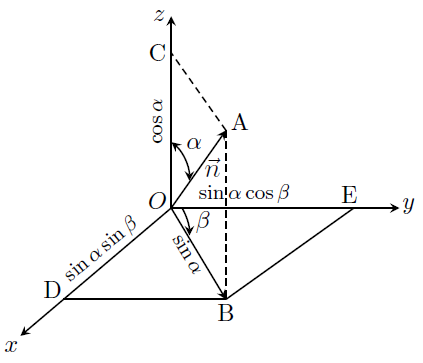
\includegraphics[width=0.45\textwidth]{coordinateaxis}
%                         ^                 ^
%                插图宽度(相对于文本宽)  插图文件名(忽略扩展名)
%% 插图标题(\label 用于设置建立交叉引用的标签名)
\bicaption{平面的倾角、倾向及其法向矢量}{Dip, dip direction and normal vector of a plane}\label{fig:samples:coordinateaxis}
\end{figure}

\figref{fig:samples:blcfy}是包含子图的例子,在\texttt{figure}环境中嵌套\texttt{subfigure}环境即可,参数格式类似,唯一不同的是\texttt{subfigure}不是一个浮动对象(被限制在\texttt{figure}中),因此其位置参数是指子图对齐的方式:\texttt{b}表示底部对齐,\texttt{t}表示顶部对齐。子图间可以用“\ltxcmdname{\textbackslash}”换行。

%% 包含子图的插图
\begin{figure}[htbp]
\def\figwidth{\columnwidth}
  \centering
    \begin{subfigure}[b]{0.58\figwidth} %子图宽度(用相对于整个figure的比例指定)
      \centering
      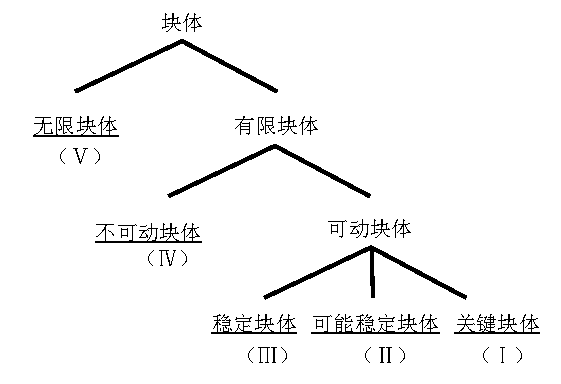
\includegraphics[width=\textwidth]{blockclassify}
      \caption{块体类型}\label{fig:samples:blockclassify}
    \end{subfigure} %此处可以用“\\”换行
    \begin{subfigure}[b]{0.4\figwidth}
      \centering
      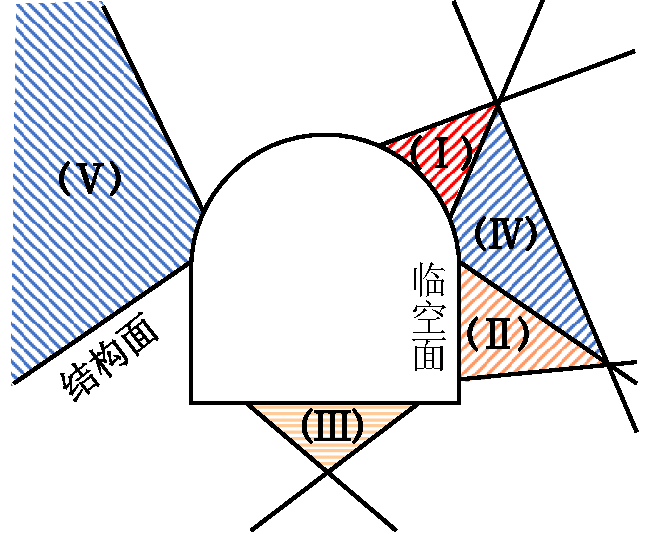
\includegraphics[width=\textwidth]{blockclassify1}
      \caption{平面示意图}\label{fig:samples:blockclassify1}
    \end{subfigure}
  \bicaption{块体分类}{Block classification}\label{fig:samples:blcfy}
\end{figure}

对于较宽的插图,可以使用“\ltxenvname{landscape}”环境按横排方式进行排版,如\figref{fig:samples:lsblcfy}所示。
\textbf{注意:}由于横排的情况下整页只有一个插图,\ltxenvname{figure}环境的位置参数一般设置为“\texttt{p}”,以保证插图纵向居中摆放。
另外,由于\ltxenvname{landscape}本身不是浮动对象,所以很可能在一页内容未排满之前遇到一个\ltxenvname{landscape}页而必须重新开始新的一页,
导致当前页提前结束排版而出现大量不必要的空白,针对此问题,可使用“\ltxenvname{afterpage}”宏包提供的“\ltxcmdname{afterpage}”命令
将\ltxenvname{landscape}页推迟到当前页排满后再开始。该命令并非$100\%$可靠,若排版结果仍然不理想,则需要进一步手工调整。

\afterpage{
%% 整页横排的插图
\begin{landscape}% 横排页环境
\pagestyle{lscape}% 横排页眉页脚样式
\begin{figure}[p]% 位置参数设置为p使得整个插图纵向居中
\def\figwidth{\columnwidth}
  \centering
    \begin{subfigure}[b]{0.5\figwidth} %子图宽度(用相对于整个figure的比例指定)
      \centering
      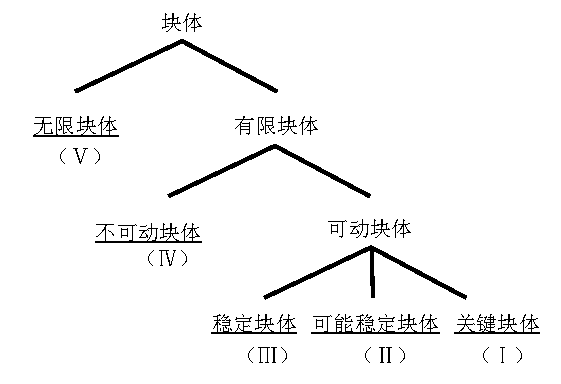
\includegraphics[width=\textwidth]{blockclassify}
      \caption{块体类型}\label{fig:samples:lsblockclassify}
    \end{subfigure} %此处可以用“\\”换行
    \begin{subfigure}[b]{0.36\figwidth}
      \centering
      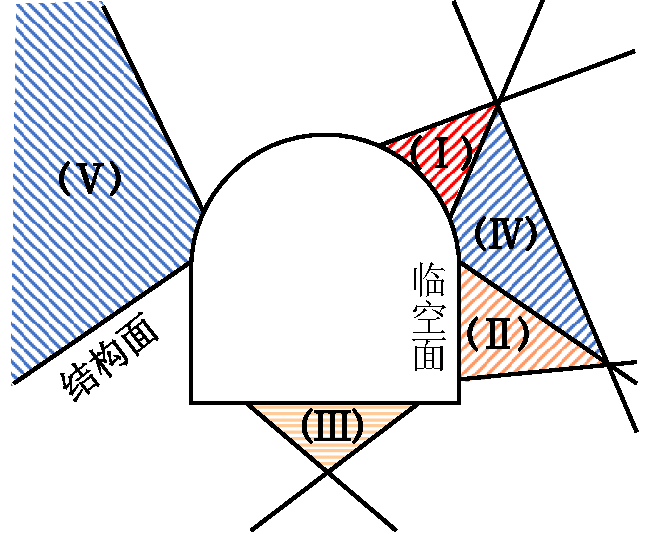
\includegraphics[width=\textwidth]{blockclassify1}
      \caption{平面示意图}\label{fig:samples:lsblockclassify1}
    \end{subfigure}
  \bicaption{块体分类(横排插图示例)}{Block classification (example for landscape figure)}\label{fig:samples:lsblcfy}
\end{figure}
\end{landscape}
}

特别注意,模版支持多种常用插图文件格式,比如\texttt{pdf}、\texttt{png}、\texttt{jpg}、\texttt{tif}等,在用\ltxcmdname{includegraphics}命令引入插图文件时,文件名可以不包含扩展名,\LaTeX{} 会自行匹配,这样做的好处是当你用另一种更好的文件格式提供同一幅插图时(比如用效果更好的矢量图格式\texttt{pdf}代替原来不够清晰的\texttt{jpg}文件),直接替换插图文件即可,正文中不需要做任何更改。

关于图表的标题,由于学校毕业论文模板要求同时给出中、英文标题,因此在排版图表标题时使用“\ltxcmdname{bicaption}”,其格式为:
\begin{verbatim}
  \bicaption[中文短标题]{中文标题}
            [Short English title]{Title in English}
\end{verbatim}
其中,方括号中的可选参数为出现在目录等其他文档结构中的标题,当图表标题很长或者包含一些不宜出现在目录中的额外标记(如文献引用标注等)时,可使用此可选参数调整呈现在目录中的标题。

\subsection{表格}\label{sec:tab}
表格和插图一样,建议使用浮动对象,即将表格放在浮动对象环境\texttt{table}中,例如\tabref{tab:samples:normal}。但是也有一些例外,例如跨页的长表格\texttt{longtable}(\tabref{tab:samples:longtable}),由于不受页面长度限制,所以不必放在浮动对象中,放进去反而会出错。

%% 普通表格
\begin{table}[htbp]
\bicaption{普通表格示例}{Sample for the normal table}\label{tab:samples:normal}
\centering
\begin{tabular}{|>{\tt}c|>{\kaishu}l|>{\tt}l|>{\kaishu}l|}
\hline
  \heiti 变量名 & \tc{\heiti 含义}    & \tc{\heiti 类型} & \tc{\heiti 备注} \\ \hline
  id           & 唯一标识符           & int             & 必须有            \\ \hline
  name         & 名称                & string          &                  \\ \hline
  abbrName     & 名称简写             & string          &                  \\
\hline
\end{tabular}
\end{table}

表格内容的输入则要比插图复杂一些,一般放在\texttt{tabular}环境中,也有的直接放在对应表格环境中(如\texttt{longtable}),列选项在表格环境参数中设置,不同的表格环境其内容大同小异。表格正文内容则一致以“\texttt{\&}”分列、以“\ltxcmdname{\textbackslash}”或“\ltxcmdname{tabularnewline}”换行。表格环境列布局的参数设置比较灵活,可以设定每一列的对齐方式(\texttt{l}、\texttt{r}或\texttt{c},有几个就有几列)、字体(放在“\texttt{>}”后的大括号内)、是否加列间线(“\texttt{|}”)等(详细说明可参考\tabref{tab:samples:longtable})。

此外,还可以使用 \ltxcmdname{multirow}、\ltxcmdname{multicolumn}等命令合并单元格,例如\tabref{tab:samples:threepart}。
\begin{enumerate}
	\item 多行单元格:\ltxcmdname{multirow\{nrows\}[bigstructs]\{width\}[fixup]\{text\}}。其中:\texttt{nrows}设定所占用的行数;\texttt{bigstructs}为可选项,主要是在使用了 bigstruct 宏包时使用;\texttt{width}设定该栏文本的宽度,如果想让 LaTeX 自行决定文本的宽度,则用 * 即可;\texttt{fixup}为可选项,主要用来调整文本的垂直位置;\texttt{text}为所要排版的文本,可用“\ltxcmdname{\textbackslash}”来强制换行。
    \item 多列单元格:\ltxcmdname{multicolumn\{ncols\}\{align\}\{text\}}。其中:\texttt{ncols}设定所占用的列数;\texttt{align}是列选项参数,类似于\texttt{tabular}环境参数,如“\texttt{|c|}”;\texttt{text}为所要排版的文本。
\end{enumerate}

此外,\tabref{tab:samples:threepart}也使用了一个特殊的表格环境\texttt{threeparttable}来生成三线表,此环境主要用处是提供了在表格内加脚注的功能,同时也预定义了一些画各种粗细线条的命令,用于生成不同粗细的表格横线。

%% 三线表及不规则单元格示例
%   (1) 跨行混排
%       \multirow{nrows}[bigstructs]{width}[fixup]{text}
%        nrows       设定所占用的行数。
%        bigstructs  此为可选项,主要是在你使用了 bigstruct 宏包时使用。
%        width       设定该栏文本的宽度。如果想让 LaTeX 自行决定文本的宽度,则用 * 即可。
%        fixup       此为可选项,主要用来调整文本的垂直位置。
%        text        所要排版的文本。可用 \\ 来强迫换行。
%   (2) 跨列混排
%       \multicolumn{ncols}{align}{text}
%        ncols  设定所占用的列数。
%        align  列选项参数,类似于tabular环境参数,如“|c|”。
%        text   所要排版的文本。
\begin{table}[htbp]
\centering
  \begin{threeparttable}
    \newcommand{\chengs}{\ensuremath{\times}}
    \newcommand{\cheng}{\ensuremath{\!\times\!}}
    \bicaption{三线表及不规则单元格示例}{Sample for the three-line table and irregular cells}\label{tab:samples:threepart}
    \begin{tabular}{cccc} %指定列数以及每列文字对齐方式:l 左对齐、r 右对齐、c 居中
      \toprule
  \multirow{2}{*}{策略}   & \multirow{2}{*}{尺寸参数}             & \multicolumn{2}{c}{数据量}    \tabularnewline \cmidrule{3-4}
                         &                                      & 数据块数\tnote{a} & 读取像素数\tnote{b} \tabularnewline \midrule
  \multirow{2}{*}{等分}   & $48\chengs 48\chengs 48$             & 2058             & 227598336 \tabularnewline \cmidrule{2-4} %从第2列到第4列画横线
                         & $128\chengs 128\chengs 128$          & 155              & 325058560 \tabularnewline \midrule
  \multirow{2}{*}{自适应} & $[16,64]\cheng[16,64]\cheng[16,64]$  & 1100             & 211624837  \tabularnewline \cmidrule{2-4}
                         & $[16,250]\cheng[16,64]\cheng[16,32]$ & 748              & 219153002  \tabularnewline %“\tabularnewline”相当于“\\”
      \bottomrule
    \end{tabular}
    \begin{tablenotes}\small
      \item[a] 每块数据包括边界
      \item[b] 第二个脚注
    \end{tablenotes}
  \end{threeparttable}
\end{table}

\texttt{longtable}环境用于排版跨页长表,与普通表格不太一样,不能当做浮动对象,当它附近有较多浮动表格对象时有可能导致表格出现的顺序和生成的编号顺序不一致,因此如无必要,建议尽量少用跨页长表,对于过长的表格应当进行适当的拆分。

%% 跨页长表
\begin{longtable}{|>{\tt}c|>{\kaishu}m{10cm}|}
  \bicaption[跨页长表示例]{跨页长表示例及表格列选项参数说明}{Sample for the long table over multiple pages and description for the parameters} \label{tab:samples:longtable}\\
    \hline \heiti 选项参数 & \tc{\heiti 说明} \\ \endfirsthead %第一页上的表头
  %% 出现在续页上的标题有两种排版方法(建议使用bicaption排版):
  % (1) 续页表格的标题、页码不出现在表格目录中,标题和表格纵向间距较小(可自行调整),注意用“\thetable”输出表格编号
  %\multicolumn{2}{c}{\bfseries\small \tablename\ \thetable\ {跨页长表示例及表格列选项参数说明(续表)}} \\
  %\multicolumn{2}{c}{\bfseries\small Table\ \thetable\ {Sample for the long table over multiple pages and description for the parameters (continued)}} \\
  % (2) 使用常规caption或bicaption排版,标题、页码将出现在表格目录中,若不想让续表出现在目录中,可将可选参数置空,如下例子所示
  %\caption[跨页长表示例(续表)]{跨页长表示例及表格列选项参数说明(续表)} \\
  \bicaption[]{跨页长表示例及表格列选项参数说明(续表)}{Sample for the long table over multiple pages and description for the parameters (continued)} \\
    \hline \heiti 选项参数 & \tc{\heiti 说明} \\ \endhead %出现在续页上的表头
    \hline         l      & 该列单元格内容左对齐 \\
    \hline         c      & 该列单元格内容居中 \\
    \hline         r      & 该列单元格内容右对齐 \\
    \hline     p\{width\} & 将内容放进一个宽为\texttt{width}的段落盒,等价于\ltxcmdname{parbox[t]\{width\}} \\
    \hline     @\{decl.\} & 删除两边列之间的空白,插入指定的文本,即大括号间的内容\texttt{decl.} \\
    \hline     m\{width\} & 指定列宽为\texttt{width},超出宽度的文字将自动换行,作用接近\ltxcmdname{parbox\{width\}} \\
    \hline     b\{width\} & 相当于\ltxcmdname{parbox[b]\{width\}} \\
    \hline     >\{decl.\} & 可在每个列选项字母之前使用,将大括号间的内容(\texttt{decl.})插入到该列每个单元格内容之前,可以用它来控制每一列的文本格式 \\
    \hline     <\{decl.\} & 可在每个列选项字母之后使用,将大括号间的内容(\texttt{decl.})插入到该列每个单元格内容之后,配合“\texttt{>}”使用可方便地将该列每个单元格放置在一个环境中,比如数学环境 \\
    \hline          |     & 插入一条竖线 \\
    \hline     !\{decl.\} & 与\texttt{|}类似,只不过插入的不是竖线而是大括号间的内容(\texttt{decl.})  \\
    \hline
\end{longtable}

对于较宽的表格,同样可以使用“\ltxenvname{landscape}”环境按横排方式进行排版,如\tabref{tab:samples:landscapelongtable}
所示,此表格也演示了在横排环境下的跨页长表排版。此处依然可以使用“\ltxcmdname{afterpage}”命令调整横排页的出现时机,
但当遇到排版程序代码的“\ltxenvname{lstlisting}”环境(本质上类似“\ltxenvname{verbatim}”环境)时有很大几率出问题,
有时甚至会导致横排页内容整体消失,因此,当横排页出现在\ltxenvname{lstlisting}附近时一般需要手工调整。

\afterpage{
\begin{landscape}% 横排页环境
\pagestyle{lscape}% 横排页眉页脚样式
\begin{longtable}{|>{\tt}c|>{\kaishu}m{10cm}|}
  \bicaption[横排跨页长表示例]{横排跨页长表示例及表格列选项参数说明}{Sample for the landscape-oriented long table over multiple pages and description for the parameters} \label{tab:samples:landscapelongtable}\\
    \hline \heiti 选项参数 & \tc{\heiti 说明} \\ \endfirsthead %第一页上的表头
  %\multicolumn{2}{c}{\bfseries\small \tablename\ \thetable\ {横排跨页长表示例及表格列选项参数说明(续表)}} \\
  %\multicolumn{2}{c}{\bfseries\small \tablename\ \thetable\ {Sample for the landscape-oriented long table over multiple pages and description for the parameters (continued)}} \\
  %\caption[横排跨页长表示例]{横排跨页长表示例及表格列选项参数说明(续表)} \\
  \bicaption[]{横排跨页长表示例及表格列选项参数说明(续表)}{Sample for the landscape-oriented long table over multiple pages and description for the parameters (continued)} \\
    \hline \heiti 选项参数 & \tc{\heiti 说明} \\ \endhead %出现在续页上的表头
    %\hline \multicolumn{2}{r}{\textit{续表见下页}}\\ \endfoot %续表脚注
    %\endlastfoot %最后一页脚注
    \hline         l      & 该列单元格内容左对齐 \\
    \hline         c      & 该列单元格内容居中 \\
    \hline         r      & 该列单元格内容右对齐 \\
    \hline     p\{width\} & 将内容放进一个宽为\texttt{width}的段落盒,等价于\ltxcmdname{parbox[t]\{width\}} \\
    \hline     @\{decl.\} & 删除两边列之间的空白,插入指定的文本,即大括号间的内容\texttt{decl.} \\
    \hline     m\{width\} & 指定列宽为\texttt{width},超出宽度的文字将自动换行,作用接近\ltxcmdname{parbox\{width\}} \\
    \hline     b\{width\} & 相当于\ltxcmdname{parbox[b]\{width\}} \\
    \hline     >\{decl.\} & 可在每个列选项字母之前使用,将大括号间的内容(\texttt{decl.})插入到该列每个单元格内容之前,可以用它来控制每一列的文本格式 \\
    \hline     <\{decl.\} & 可在每个列选项字母之后使用,将大括号间的内容(\texttt{decl.})插入到该列每个单元格内容之后,配合“\texttt{>}”使用可方便地将该列每个单元格放置在一个环境中,比如数学环境 \\
    \hline          |     & 插入一条竖线 \\
    \hline     !\{decl.\} & 与\texttt{|}类似,只不过插入的不是竖线而是大括号间的内容(\texttt{decl.})  \\
    \hline
\end{longtable}
\end{landscape}
}

跨页表格的标题与一般表格不同,需额外提供续表标题,排版格式如下:
{\linespread{1.2}
\begin{verbatim}
  \bicaption[短标题]{标题}[Short title]{Title} \label{...} \\
    \hline 列名1 & 列名2 & ... \\ \endfirsthead %第一页上的表头
  \bicaption[短标题(续表)]{标题(续表)}
            [Short title (continued)]{Title (continued)} \\
    \hline 列名1 & 列名2 & ... \\ \endhead %出现在续页上的表头
\end{verbatim}}
按上述方式排版,续表标题及页码将出现在表目录中,若不想要这样的效果,可以将续表标题“\ltxcmdname{bicaption}”命令的可选参数置空(注意要保留“\texttt{[]}”)。

\subsection{定理}
定理,包括命题、引理、推论等的排版使用 \texttt{theorem}、\texttt{lemma}、\texttt{proposition} 等环境,每个定理可用可选参数指定一个别名。定理的证明放在 \texttt{proof} 环境中,证明结束标志为 \ltxcmdname{qedhere}。

定理示例:
\begin{theorem}[有限性定理] \label{thm:samples:t}
块体为有限的充分必要条件是节理锥(JP)与开挖锥(EP)的交集为空集。
\end{theorem}

公理示例:
\begin{axiom} \label{thm:samples:a}
平面上两点确定一条直线。
\end{axiom}

引理示例:
\begin{lemma} \label{thm:samples:l}
块体为有限的充分必要条件是节理锥(JP)与开挖锥(EP)的交集为空集。
\end{lemma}

命题及证明示例:
\newcommand{\sNP}{\ensuremath{\mathcal{NP}}}
\newcommand{\tNP}{\sNP\ }
\newcommand{\tNPC}{\mbox{\ensuremath{\mathcal{NP}\text{-完全}}}}
\begin{proposition} \label{thm:samples:p}
若有向图的哈密尔顿环路问题是~\tNPC 问题,则无向图的哈密尔顿环路问题也是~\tNPC 问题。
\end{proposition}

\begin{proof}
    显然,无向哈密尔顿环路问题属于~\tNP 问题,因此只要证明有向图的哈密尔顿环路问题可多项式规约到无向图的
    哈密尔顿环路问题~(已知有向图的哈密尔顿问题是~\tNPC 问题)。

    令~$G=(V,E)$ 是包含~$n$ 个顶点的有向图,现将其转换到无向图~$G'=(V',E')$:对每个~$v\in V$,
    $V'$ 中包含~$3$ 个顶点~$v^1,v^2,v^3$ 与之对应,$E'$ 中包含两条无向边~$v^1v^2,v^2v^3$ 与之对应,
    对~$E$ 中的每条边~$vw$,$E'$ 中包含无向边~$v^3w^1$ 与之对应,显然,该转换所需时间以多项式为界,
    若~$|V|=n,|E|=m$ 则~$|V'|=3n,|E'|=2n+m$。

    若~$G$ 中有一条有向哈密尔顿环路~$v_1,\cdots,v_n$,则~$v_1^1,v_1^2,v_1^3,v_2^1,v_2^2,v_2^3,\cdots,$ $v_n^1,v_n^2,v_n^3$ 是~$G'$ 中
    的一条~(无向) 哈密尔顿环路;另一方面,若~$G'$ 中存在一条哈密尔顿环路,由于对每组顶点~$v^1,v^2,v^3$,$v^2$ 只与~$v^1$ 和~$v^3$ 相连,
    因此在环路上必按~$v^1,v^2,v^3$ 或~$v^3,v^2,v^1$ 的顺序访问这三个顶点,而~$G'$ 中的其他边仅连接上标为~$1$ 和~$3$ 的顶点,
    因此该环路上所有的三顶点组要么都按~$1,2,3$ 的顺序排列,要么都按~$3,2,1$ 的顺序排列,
    不妨设该环路为~$v_{i_1}^1,v_{i_1}^2,v_{i_1}^3,\cdots,v_{i_n}^1,v_{i_n}^2,v_{i_n}^3$,则~$v_{i_1},\cdots,v_{i_n}$ 是~$G$ 中的一条
    有向哈密尔顿环路。所以~$G$ 包含有向哈密尔顿环路当且仅当~$G'$ 包含无向哈密尔顿环路。\qedhere
\end{proof}

定义示例:
\begin{definition}[复流形] \label{thm:samples:d}
复流形$M$是一个可微流形,它容许一个开覆盖$\{U_{\alpha}\}$和坐标映射$\varphi_{\alpha}:U_{\alpha}\rightarrow \mathbb{C}^n$ 使得对所有的$\alpha, \beta, \varphi_{\alpha}\circ \varphi_{\beta}^{-1}$在$\varphi_{\beta}(U_{\alpha}\cap U_{\beta})\subset \mathbb{C}^n$是全纯的。
\end{definition}

\subsection{算法}

如\algoref{alg:euclid}所示,详细使用方法请参见文档 \href{https://ctan.org/pkg/algorithmicx?lang=en}{algorithmicx}。

\begin{algorithm}[htbp]
    \small
    \caption{Euclid's algorithm}\label{alg:euclid}
    \begin{algorithmic}[1]
        \Procedure{Euclid}{$a,b$}\Comment{The g.c.d. of a and b}
        \State $r\gets a\bmod b$
        \While{$r\not=0$}\Comment{We have the answer if r is 0}
        \State $a\gets b$
        \State $b\gets r$
        \State $r\gets a\bmod b$
        \EndWhile\label{alg:euclid:while}
        \State \textbf{return} $b$\Comment{The gcd is b}
        \EndProcedure
    \end{algorithmic}
\end{algorithm}

对算法内某一行的引用:\algoref{alg:euclid}中第~\ref{alg:euclid:while} 行。

\subsection{计算机程序}
计算机源程序可以用 \texttt{lstlisting} 环境排版,代码可直接拷贝进去,除语法高亮外基本原样输出。下面是一个简单的例子:
\begin{lstlisting}
  int PacketQueue::put(AVPacket *pkt) {
      int ret;    
      this->mutex->lock();
      ret = put_private(pkt);
      this->mutex->unlock();    
      if (pkt != &this->flush_pkt && ret < 0) av_packet_unref(pkt);    
      return ret;
  }
\end{lstlisting}

本模版预设按C++语法进行排版及关键字高亮显示,可以用环境参数中切换语言并作其他更细致的设定,例如 \texttt{[language=Pascal]} 将当前 \texttt{lstlisting} 环境切换为 Pascal 语言。同时,也可以通过参数设置将其变为浮动对象:\texttt{[float, caption=A floating example]},如 \codref{lst:samples:pas} 所示。更详细的用法可参考 \texttt{listings} 宏包的说明文档(\texttt{listings.pdf})。
\begin{lstlisting}[float, language=Pascal, caption={浮动代码块}, label={lst:samples:pas}]
  var i:integer;
  var x:integer;
  for i:=maxint to 0 do
  begin
    if (i<=0) then x := 1;
    if (i>0) then x := 0;
  end;
\end{lstlisting}

\subsection{交叉引用}
理论上在文档的任何位置都可以设置交叉引用点,常用的有:特定章节、图、表、公式等。为被引用对象建立交叉引用点的方法是在相应位置使用 \ltxcmdname{label}命令设置一个标签,在需要引用的地方用 \ltxcmdname{ref} 命令建立引用链接,其参数就是前面所设置的标签名称。例如:参见 \ref{sec:samples} 节。由于引用链接只输出\LaTeX{} 为标签自动生成的编号,所以一般要在 \ltxcmdname{ref} 命令的前后配上相应文字,如“图”、“表”、“公式”等。为省去此琐碎环节,本模版预定义了一些固定的引用模式供大家使用,如:章节引用\secref{sec:samples}、插图引用\figref{fig:samples:blcfy}、表格引用\tabref{tab:samples:normal}、算法引用\algoref{alg:euclid}、代码引用\codref{lst:samples:pas}、定理引用\thmref{thm:samples:t}、公理引用\axmref{thm:samples:a}、引理引用\lemref{thm:samples:l}、命题引用\prpref{thm:samples:p}、定义引用\defref{thm:samples:d}等。

另外,还可以使用 \ltxcmdname{pageref}引用对象所在页码,例如:\figref{fig:samples:blcfy}在第 \pageref{fig:samples:blcfy} 页。

页面内的脚注用 \ltxcmdname{footnote}命令添加,例如:此处\footnote{脚注内容。}有脚注。

\subsection{参考文献引用}\label{sec:samples:cite}
模板提供了一组源自\texttt{natbib}包的引用命令用于不同风格的引用习惯:
\begin{center}
%\linespread{0.5}
%\renewcommand{\arraystretch}{1.0}
\begin{tabular}{lcl}
\verb|\citet{wikibook2014latex}| & $\Rightarrow$ & \citet{wikibook2014latex} \\
\verb|\citet[第2章]{wikibook2014latex}| & $\Rightarrow$ & \citet[第2章]{wikibook2014latex} \\
\verb|\citep{wikibook2014latex}| & $\Rightarrow$ & \citep{wikibook2014latex} \\
\verb|\citep[第2章]{wikibook2014latex}| & $\Rightarrow$ & \citep[第2章]{wikibook2014latex} \\
\verb|\citep[见][第2章]{wikibook2014latex}| & $\Rightarrow$ & \citep[见][第2章]{wikibook2014latex}
\end{tabular}
\end{center}

其中,后缀“\texttt{t}”表示“textual”,即句中(文本中的)引用,也就是引用本身是句子的一个成分,去掉引用句子就不通了;
后缀“\texttt{p}”表示“parenthetical”(括号里的),即句中插入说明或句末引用,作为一个插入语(附加说明)存在,非句子成分,去掉引用句子仍然是完整通顺的。请自行体会其中的区别。

但以上命令主要为英文文献设计,有些地方并不是很符合中文的习惯。在中文文献中,若使用数字序号形式的引用标注,
句末引用一般采用上标形式,句中引用则仍使用正常形式。但在基础模板中,虽然提供了“\texttt{super}”文档参数支持上标形式的引用标注,
但却是一股脑把所有标注命令全改成上标形式,不是很合理。因此,若采用数字序号形式的引用标注,必要时可直接用“\ltxcmdname{cite}”命令自行排版。

为便于后期统一修改引用标注风格,建议根据自己的需要自行定义相关命令,简化论文撰写过程,例如在“\texttt{Thesis.tex}”文件的导言区或“\texttt{artracom.sty}”
加入相关自定义命令:{\linespread{1.1}
\begin{verbatim}
  \newcommand*{\ntcite}[1]{~\cite{#1}~}
  \newcommand*{\npcite}[1]{\textsuperscript{\cite{#1}}}
\end{verbatim}}
用于生成不同位置的文献引用标注,此处文献\ntcite{wikibook2014latex}是句中引用(文献本身是句子成分之一),这是句中\npcite{wikibook2014latex}插入引用,这是句末(文献不是句子成分之一,仅表示名词或句子来自哪篇文献)引用\npcite{wikibook2014latex}。

参考文献信息记录在“\texttt{.bib}”文件中,务必保证每一条文献信息完整、准确,建议用开源软件~\href{https://www.jabref.org/}{JabRef}~进行信息录入和管理。

\section{简要写作指南}

\subsection{摘要的写法}

摘要是全文的高度概括和浓缩,一般为“三段式”结构,即:开头、展开、结尾。

\textbf{开头段}:精练说明研究背景和目的;

\textbf{展开段}:进一步阐明论文的内容,包括研究方法和研究成果,
要归纳提炼出论文完成的主要工作成果、特色及其创新点等,简单地可采用但不必拘泥于如下形式:

本文完成的主要工作如下:
\begin{enumerate}
\item 研究了……
\item 提出了……
\item 完成了……
\end{enumerate}

\textbf{结尾段}:给出研究的主要结论,并指出论文工作的价值和意义。

论文摘要写作应避免过于简短、句子结构太呆扳以及使用非规范的缩略语,不要出现疑问句和感叹句。

\textbf{中文摘要}力求语言精炼准确,硕士论文一般为1000字左右(以汉字计),博士论文可以稍长一些,但是最好也不要超过2000字。
摘要中不要出现插图或表格等内容,也不要出现参考文献引用。所有外文缩写首次出现必须给出全称。

\textbf{英文摘要}内容与中文摘要相对应,在语法、用词上应准确无误,但必须避免生硬的逐字、逐句机械地转换成英语,形成带有明显汉语痕迹的Chinglish(中式英语)。
这里推荐阅读一位美国的专利审核员Felicia L. Brittman女士在阅读了200多篇中国工科学生撰写的英文论文后总结出的一篇“常见错误合辑”:
“\textit{The Most Common Habits from more than 200 English Papers written by Graduate Chinese Engineering Students}”。
这篇文章的作者曾于2002年到2003年期间在上海交通大学担任客座讲师,并通晓汉语,这一背景使得她的这篇文章非常具有针对性,且具有很高的参考价值。
另外,可合理利用一些英文翻译和润色工具对英文摘要进行进一步修改完善,例如\href{https://www.deepl.com/}{DeepL}、\href{https://www.grammarly.com/}{Grammarly}等。

最后是关键词的选取。关键词是指论文中最主要、最关键的、重复率最高的词或词组,多选择名词或名词性短语,数量一般为5个左右。
关键词的功能在于使读者据名猜意,了解全篇主旨,并方便论文检索,一般可从论文标题和摘要中选取。

\subsection{文献综述的写法}

在学位论文中,一般有两处地方涉及文献综述。其一是在论文第1章绪论中有一节“国内外研究现状”,其二一般是第2章整个一章作为相关理论和方法的综述。
后者在博士学位论文中比较常见,硕士学位论文如果综述篇幅较短,一般将内容都放到第1章中,而不再出现单独的一章用于综述。

在这两部分同时存在的情况下,不能将其视为同样的内容,或者仅仅是简略和详细的差别,更不能在有独立的第2章综述的情况下省略第1章的“国内外研究现状”。
两者各有侧重,写法不同。前者是对论文研究背景下相关理论、方法、应用等方面发展现状的全方位概述,重点突出目前各个方向研究前沿的状况
(即目前最好的方法、最广泛的应用等),注重“面”的叙述;后者则是对与论文研究内容密切或直接相关的理论和方法的论述和分析,注重“点”的叙述,需要具体、深入,
且具有较强的针对性,同时应当指出已有方法存在的问题或缺陷,并能够直接引出后续章节的研究内容。若论文不设独立的综述章,则第1章的“国内外研究现状”
部分应承担后者类似的功能。

文献综述内容的撰写要注意完整性和逻辑性,相关工作可按照研究的不同阶段(时间先后)或不同特点分类整理归纳。文献的选择要有针对性和目的性,
不要把看过的文献不加筛选地都塞到论文中;同时也要有自己的分析和评述,切忌大段摘抄和简单罗列。

文献综述应当有一个总结性的结尾,其内容一般以现存问题和发展方向为主,要避免出现“戛然而止”没有下文的情况。

\subsection{核心章的写法}

学位论文的核心章一般是对论文主要工作及成果的叙述,每一项工作用独立的一章来叙述。在撰写核心章之前需要对整个论文的框架有一个基本的把握,
核心章的前后顺序和联系要能够体现出论文工作的整体性和逻辑性,最好在第1章“研究内容”部分将这个整体框架讲清楚,建议画一个逻辑框图来辅助叙述。

核心章的开头一般用一小段引言(不分节不编号)来连接上文并引出下文,起到一个承上启下的作用,以进一步增强论文的整体性。核心章结构切忌千篇一律,例如:
第1节“概述”、第2节“……算法”、第3节“实验及分析”、第4节“本章小结”。除了“本章小结”是固定的之外,其他小节都可以体现出这一章的特殊性。
比如上面例子中的第2节,由于整个一章其实都是在说这个算法,“……算法”这个小节标题就显得多余而毫无意义,完全可以把这一节下一级的小节都提升一级,
直接作为这一章的小节来安排。核心章结构建议按照该章所要叙述方法的关键环节、特点或创新点来分节,从而避免出现各个核心章的结构雷同。

核心章的内容以论文工作叙述为主,不要再对已有方法作大篇幅的介绍,如果必须要提及已有方法(例如论文方法是对某些已有方法的改进),则在介绍已有
方法时必须密切配合论文工作本身来做有针对性的叙述,而不能再做一般性的介绍,一般性的介绍应该放到前面的综述环节去做。

\subsection{结论与展望的写法}

最后一章“结论与展望”一般分成“结论”和“展望”两节。

“结论”部分是对整个论文工作的完整和详细的总结,着重阐述论文的独创性工作以及所取得的研究成果,包括在研究过程中发现的一些结论性的客观现象或规律。
另外,还可以对论文工作成果在相关研究领域的地位、作用和意义进行一番阐述。这一部分可参考摘要的框架去写,但是不要照搬摘要内容。
实际上这部分内容在论文工作成果的叙述上一般要比摘要更具体深入,同时在叙述范围上也会更广泛一些,会包含摘要没有涵盖的部分内容,例如一些结论性的描述。

“展望”部分主要是基于论文的工作成果进一步提出需要讨论的问题和建议,也可以对相关领域的未来研究方向展开讨论。这一部分切勿写成对论文工作存在不足的“检讨”,
原则上,学位论文是对你研究生阶段研究工作的一个总结,如果还存在明显的“不足”或“缺陷”,则说明论文的工作尚没有完成,在这个情况下申请答辩是存在问题的。

%!TEX root = ../Thesis.tex
%!Mode:: "TeX:UTF-8"

\chapter{中国科学院大学研究生学位论文撰写规范指导意见(节选)}

学位论文是研究生在掌握已有的科学知识的基础上,运用科学思维和一定的科学方法、技术与工具,面向特定的科学领域所存在的科学问题,开展创新性研究而产生的科学研究成果。

学位论文是研究生科研工作成果的集中体现,是评判学位申请者学术水平、授予其学位的主要依据,是科研领域重要的文献资料。撰写学位论文是对研究生科学研究能力的基本训练,是研究生学业与研究成效的基本检验,也是科研与创新能力的重要体现。

为提高研究生学位论文的撰写质量,促进学位论文在内容和格式上的规范化,参照《学位论文编写规则》(GB/T 7713.1—2006)、《信息与文献 参考文献著录规则》(GB/T 7714—2015)和《学术出版规范 期刊学术不端行为界定》(CY/T 174—2019)等国家有关标准,特制定本指导意见(2021年修订)。各学科群学位评定分委员会(以下简称各学科群分会)可结合本学科领域的特点,参考本指导意见,制订符合本学科领域特点与要求的学位论文撰写具体要求。

本指导意见从2023年冬季批次开始实施。

\section{组成及要求}
学位论文一般由以下几个部分组成:封面、原创性声明及授权使用声明、摘要、目录、符号说明(若有)、正文、参考文献、附录(若有)、致谢、作者简历及攻读学位期间发表的学术论文与其他相关学术成果等。
\subsection{封面}
一律采用中国科学院大学规定的统一中英文封面,封面包含内容如下:

\begin{enumerate}
    \item 密级,涉密或延迟公开论文必须在论文封面标注密级,同时注明保密年限。公开论文不标注密级,可删除此行。
    \item 论文题目,应简明扼要地概括和反映整个论文的核心内容,一般不宜超过25个汉字(符),英文题目一般不应超过150个字母,必要时可加副标题。题目中应尽量避免使用缩略词、首字母缩写词、字符、代号和公式等。
    \item 作者姓名,根据《中国人名汉语拼音字母拼写规则》(GB/T 28039—2011),英文封面中的姓和名分写,姓在前,名在后,姓名之间用空格分开。姓和名需写全拼,姓全大写,名首字母大写。外国留学生姓名书写顺序以护照格式为准,字母全部大写。
    \item 指导教师,需同时填写导师姓名、专业技术职务和工作单位。如果有多位导师(均需经培养单位批准,并在学籍系统备案),第一导师在前,第二导师等依次在后。学位论文在指导小组的指导下完成的,应注明指导小组成员相应信息。
    \item 学位类别,包括学科门类(学术型)或专业学位类别以及学位级别。学科门类如理学、医学等,专业学位类别如应用统计、工商管理等。学位级别包括硕士、博士。
    \item 学科专业,填写攻读学位的一级学科/二级学科或专业学位类别/领域全称,须与学籍信息一致,不可用简写。
    \item 培养单位,填写就读研究所或学院、系全称,如中国科学院××研究所、中国科学院大学××学院。
    \item 时间,填写论文提交学位授予单位的年月,使用阿拉伯数字标注。一般夏季申请学位的论文标注6月,冬季申请学位的论文标注12月。例如:2023年6月,2023年12月。
\end{enumerate}

\subsection{原创性声明及授权使用声明}
本部分内容提供统一的模版,提交时作者和导师须亲笔签名。如遇导师无法签字时,培养单位应做出适当处理。
\subsection{摘要和关键词}
论文摘要包括中文摘要和英文摘要(Abstract)两部分。论文摘要应概括地反映出本论文的主要内容,说明本论文的主要研究目的、内容、方法、结论。要突出本论文的创造性成果或新见解,不宜使用公式、图表、表格或其他插图材料,不标注引用文献。中文摘要的字数由各学科群分会根据本分会涉及学科专业的特点提出具体要求。英文摘要与中文摘要内容应保持一致。留学生用其他语种撰写学位论文时,应有详细的中文摘要,字数由各学科群分会具体制定,建议一般不少于5000字。

摘要最后注明本文的关键词(3~5个)。关键词是为了文献标引和检索工作,从论文中选取出来,用以表示全文主题内容信息的单词或术语。关键词以显著的字符另起一行并隔行排列于摘要下方,左顶格,中文关键词间用中文逗号隔开。英文关键词应与中文关键词对应,首字母应大写,用英文逗号隔开。

摘要应另起一页,与正文前的内容连续编页(用罗马字符)。
\subsection{目录}
目录应包括论文正文中的全部内容的标题,以及参考文献、附录(若有)和致谢等,不包括中英文摘要。目录页由论文的章、条、附录等序号、名称和页码组成。正文章节题名要求最多编到第三级标题,即×.×.×(如1.1.1)。一级标题顶格书写,二级标题缩进一个汉字符位置,三级标题缩进两个汉字符位置。论文中若有图表,应有图表目录,置于目录页之后,另页编排。图表目录应有序号、图题或表题和页码。

目录应另起一页,与正文前的内容连续编页(用罗马字符)。
\subsection{符号说明(若有)}
如果论文中使用了大量的物理量符号、标志、缩略词、专门计量单位、自定义名词和术语等,应编写成注释说明汇集表。若上述符号等使用数量不多,可以不设此部分,但必须在论文中首次出现时加以说明。
论文中若有符号说明,应置于目录之后、正文之前,另起一页,与正文前的内容连续编页(用罗马字符)。
\subsection{正文}
正文一般包括绪论、论文主体、研究结论与展望等部分。

\begin{enumerate}
    \item 绪论应包括选题的背景和意义,国内外相关研究成果与进展述评,本论文所要解决的科学与技术问题、所运用的主要理论和方法、基本思路和论文结构等。绪论应独立成章,用足够的文字叙述,不与摘要雷同。要实事求是,不夸大也不弱化前人的工作和自己的工作。
    \item 论文主体是正文的核心部分,占主要篇幅,它是将学习和研究过程中调查、观察和测试所获得的材料和数据,经过思考判断、加工整理和分析研究,进而形成论点。依据学科专业及具体选题,论文主体可以有不同的表现形式,可以按照章与节的结构表述,也可以按照“研究背景与意义—研究方法与过程—研究结果与讨论”的表述形式组织论文。但主体内容必须实事求是,客观诚实,准确完备,合乎逻辑,层次分明,简明可读。
    \item 研究结论是对整个论文主要成果的总结,不是正文中各章小结的简单重复,应准确、完整、明确、精炼。应明确凝练出本研究的主要创新点,对论文的学术价值和应用价值等加以分析和评价,说明本项研究的局限性或研究中尚难解决的问题,并提出今后进一步在本研究方向进行研究工作的设想或建议。结论部分应严格区分本人研究成果与他人科研成果的界限。
\end{enumerate}
\subsection{参考文献}
本着严谨求实的科学态度撰写论文,凡学位论文中有引用或参考、借鉴他人思想或成果之处,均应按一定的引用规范,列于文末(通篇正文之后),参考文献部分应与正文的文献引用一一对应,注重合理引用,严禁抄袭剽窃等学术不端行为。
\subsection{附录(若有)}
主要列入正文内过分冗长的公式推导、供查读方便所需的辅助性数学工具或表格、数据图表、程序全文及说明、调查问卷、实验说明等。
\subsection{致谢}
对给予各类资助、指导和协助完成研究工作,以及提供各种对论文工作有利条件的单位及个人表示感谢。致谢应实事求是,切忌浮夸与庸俗之词。致谢末尾应具日期,日期与论文封面一致。
\subsection{作者简历及攻读学位期间发表的学术论文与其他相关学术成果}
作者简历应包括从大学起到申请学位时的个人学习工作经历。按学术论文发表的时间顺序,列出作者本人在攻读学位期间发表或已录用的学术论文清单(著录格式同参考文献)。其他相关学术成果可以是申请的专利、获得的奖项及完成的项目等代表本人学术成就的各类成果。


\section{撰写要求}

\subsection{学位论文基本要求}
学位论文必须是一篇系统的、完整的学术论文,遵循既定的学术规范与要求,不仅要符合学位论文的形式规范,更要符合学位论文的质量规范。做到:学术观点明确,立论正确,方法科学,材料翔实,数据可靠,推理严谨,论证充分,引用规范,结构合理,层次分明,文字通顺,表达准确,学风严谨。研究成果体现作者独到的学术见解、科学论证与创新性结论,表明作者掌握了坚实的基础理论和系统的专门知识,具有独立地从事科学研究的能力。

硕士学位论文选题应为本学科重要领域,有一定的理论意义或应用价值;在理论或方法上有一定的创新,解决了科学或生产实践中某一项重要的问题,取得重要的研究成果,具有较好的社会效益或应用前景。

博士学位论文选题应为本学科前沿领域,有重要的理论意义或应用价值;在理论或方法上有较大的创新,解决了科学或生产实践中某一项重大的问题,取得突破性的研究成果,具有重要的社会效益或应用前景。

\subsection{论文原创性要求}

学位论文应为学位申请者在导师的指导下独立完成的科学研究成果,为作者本人的原创性成果,系研究生经过多年的专业学习和科学研究,运用科学思维、科学方法或工具,探索科学领域中的某一科学问题,提出问题,分析问题,解决问题。学位论文中要有清晰完整的文献综述,但不能以文献综述来代替学位论文。论文引用规范合理,没有伪造、篡改、剽窃、他人代写、论文买卖及其它学术不端行为。

\subsection{论文创新性要求}

学位论文的研究既包括创造知识,即创新、发现和发明,是对未知世界及其规律的探索,也包括整理知识,即对已有知识分析整理,使其规范化、系统化,是对已有知识的传承。创新活动,贯穿了学位论文研究与写作的全过程,如提出新的学术思想、科学概念、假说、学说、定理、定律,设计新的观察方法和实验手段,建立新的科学模型,研制出新的产品,设计出新的工艺流程,发现新的物种等。学位论文的价值在于探索未知,发现科学发展中的规律与特征。学位论文要体现其应有的严谨性与探索性,在原创性的基础上实现对已有知识的超越、突破或颠覆,发现前所未有的科学问题,提出前所未有的分析论证,得出前所未有的科学结论。

\subsection{学位论文的字数要求}
学位论文最重要的意义在于其学术研究的创新性,应将学位论文的质量水平作为主要考量,不以字数多少作为特别要求,但各学科群分会可根据本领域涉及的学科专业特点做相应规定。

\subsection{文字、标点符号和数字}

除外国来华留学生、外语专业研究生以及特殊需要外,学位论文一律用国家正式公布实施的简化汉字书写。标点符号的用法以《标点符号用法》(GB/T 15834—2011)为准。数字用法以《出版物上数字用法》(GB/T 15835—2011)为准。

外国来华留学生可用中文或英文撰写学位论文,但应有详细的中英文摘要。外语专业的学位论文应用所学专业相应的语言撰写,摘要应使用中文和所学专业相应的语言对照撰写。

为了便于国际合作与交流,中文学位论文亦可有英文或其他文字的副本。

\subsection{论文正文}

\subsubsection{章节和各章标题}
论文正文须由另页右页(奇数页)开始,用阿拉伯数字连续编码,一直到全文最后。正文内部新章节无须另页右页(奇数页)开始。
    论文可参考“绪论-研究背景与意义-研究方法与过程-研究结果与讨论-研究结论与展望”的结构形式撰写,各主体研究内容可分别单独成为章节并作为章节标题使用。

各章标题中尽量不采用英文缩写词,对必须采用者,应使用本行业的通用缩写词。标题中尽量不使用标点符号。
\subsubsection{序号}
\textbf{标题序号}

论文标题分层设序。层次以少为宜,根据实际需要选择。各层次标题一律用阿拉伯数字连续编号。以三级标题为宜,最多四级。若确需要再增加一级,以小括号形式表示;不同层次的数字之间用小圆点“.”相隔,末位数字后面不加点号,如“1.1”,“1.1.1”等;章的标题居中排版,各层次的序号均左起顶格排,序号与题名间空一个汉字符。

\textbf{图表等编号}

论文中的图、表、附注、公式、算式等,一律用阿拉伯数字分章依序连续编码。其标注形式应便于互相区别,如:图1-1(第1章第一个图)、图2-2(第2章第二个图);表3-2(第3章第二个表)等。附录的图表参考正文的编号方式,如附图1-1或附表1-1。

\textbf{页码}

正文页码从绪论开始按阿拉伯数字(1,2,3……)连续编排,页码应位居左页左下角、右页右下角;正文前的部分(中英文摘要、目录等)用大写罗马数字(I,II,III…)单独编排,页码位于页面下方居中。
\subsubsection{页眉}
页眉从摘要开始,奇数页上标明“摘要”、“Abstract”、“目录”、“图表目录”等,偶数页上标明论文题目(英文摘要标明英文题目)。正文(即第1章开始到最后一章)的页眉,奇数页上标明每一章名称,偶数页上标明论文题目。参考文献、附录、致谢等的页眉,奇数页标明“参考文献”、“附录”、“致谢”等,偶数页标明论文题目。页眉居中设置。

\subsubsection{名词和术语}
科技名词术语及设备、元件的名称,应采用全国科学技术名词审定委员会公布的权威标准或其他相关权威信息源规定的术语或名称。标准中未规定的术语要采用行业通用术语或名称。全文名词术语必须统一。一些特殊名词或新名词应在适当位置加以说明或注解。双名法的生物学名部分均为拉丁文,并为斜体字。

采用英语缩写词时,除本行业广泛应用的通用缩写词外,文中第一次出现的缩写词应该用括号注明英文原词。新的外来名词应用括号注明英语全称和缩写语。

\subsubsection{量和单位}

量和单位要严格执行《国际单位制及其应用》(GB 3100-93)、《有关量、单位和符号的一般原则》(GB3101—93)有关量和单位的规定。量的符号一般为单个拉丁字母或希腊字母,并一律采用斜体(pH例外)。

\subsubsection{图和表}

论文中若有图和表,应设置图表目录,先列图后列表,置于目录页后,另页编排。

\textbf{(1) 图}

图片大小适当,图边界在页面范围内(图边界离页面边界距离大于页边距)。若图片中包含文字,文字大小不超过正文文字大小。
图包括曲线图、构造图、示意图、框图、流程图、记录图、地图、照片等,宜插入正文适当位置。引用的图必须注明来源。具体要求如下
\begin{itemize}
    \item 图应具有“自明性”,即只看图、图题和图注,不阅读正文,就可理解图意。每一图应有简短确切的图题,连同图序置于图下居中。
    \item 图中的符号标记、代码及实验条件等,可用最简练的文字横排于图框内或图框外的某一部位作为图注说明,全文统一。图题建议用中文及英文两种文字表达。
    \item 照片图要求主要显示部分的轮廓鲜明,便于制版,如用放大、缩小的复制品,必须清晰,反差适中,照片上应有表示目的物尺寸的标尺。
    \item 图片一般设为高6cm×宽8cm,但高、宽也可根据图片量及排版需要按比例缩放。中文(宋体)英文(Times New Roman)图注为五号字,1.25倍行距。
    \item 文中尽量不用世界地图、全国地图!如果一定要用,凡涉国界图件(国内部分地区、全国、世界部分地区、全球)必须使用自然资源部标准地图底图(下载网址:http://bzdt.ch.mnr.gov.cn),所用底图边界要完全无修改(包括南海诸岛位置),为适应排版时图的缩放,比例尺一律用线段比例尺,而不用数字比例尺。并在图题下注明“注:该图基于自然资源部标准地图服务网站下载的审图号为GS(2021)××××号的标准地图制作,底图边界无修改。”
\end{itemize}


\textbf{(2) 表}

表的编排一般是内容和测试项目由左至右横读,数据依序竖排,应有自明性,引用的表必须注明来源。具体要求如下:
\begin{itemize}
    \item 每一表应有简短确切的题名,连同表序置于表上居中。必要时,应将表中的符号、标记、代码及需说明的事项,以最简练的文字横排于表下作为表注。表题建议用中文及英文两种文字表达。
    \item 表内同一栏数字必须上下对齐。表内不应用“同上”、“同左”等类似词及“″”符号,一律填入具体数字或文字,表内“空白”代表无此项,“—”或“…”(因“—”可能与代表阴性反应相混)代表未发现,“0”该表实测结果为零。表内未测出值可以用“N.D. ”表示。
    \item 表格尽量用“三线表”,避免出现竖线,避免使用过大的表格,确有必要时可采用卧排表,正确方位应为“顶左底右”,即表顶朝左,表底朝右。表格太大需要转页时,需要在续表表头上方注明“续表”,表头也应重复排出。
    \item 中文(宋体)英文(Times New Roman)表注为五号字,1.25倍行距。
\end{itemize}

\subsubsection{表达式}
论文中的表达式需另行起,原则上应居中。若有两个以上的表达式,应从“1”开始的阿拉伯数字进行编号,并将编号置于括号内。编号采用右端对齐。表达式较多时可分章编号。

较长的表达式如必须转行,只能在+,-,×,÷,<,>等运算符之后转行,序号编于最后一行右顶格。

\subsection{参考文献}
参考文献格式规范参照《信息与文献 参考文献著录规则》(GB/T 7714—2015),或可参照国际刊物通行的参考文献格式。各学科群分会可根据本学科的一般规范制定相应的参考文献格式。文后参考文献和参考文献在正文中的标注方式可采用“顺序编码制”或“著者—出版年制”。确定采用某种方法后,文后参考文献和参考文献在正文中的标注方式要对应。

文后参考文献按“顺序编码制”组织时,各篇文献应按正文部分首次引用时标注的序号依次列出;文后参考文献按“著者—出版年制”组织时,条目不排序号,先按语种分类排列,语种顺序是:中文、日文、西文、俄文、其他文种;然后按著者字序和出版年排列。中文和日文按第一著者的姓氏笔画排序,中文也可按汉语拼音字母顺序排列,西文和俄文按第一著者姓氏字母顺序排列。当一个著者有多篇文献并为第一著者时,该著者单独署名的文献排在前面(并按出版年份的先后排列),接着排该著者与其他人合写的文献。
文后参考文献加标题“参考文献”,并列入全文目录。
凡正文里标注了参考文献的,其文献都必须列入文后参考文献。文后参考文献应集中著录于正文之后,不分章节著录。
正文中未被引用但被阅读或具有补充信息的文献可集中列入附录中,其标题为“荐读书目”。

详细内容请参考《中国科学院大学研究生学位论文撰写规范指导意见》。

\section{排版与印刷要求}

\subsection{纸张与页面要求}
\begin{table}[h]
    \centering
        \bicaption{排版和印刷要求}{Typography and Printing Requirements}
    \begin{tabular}{lc}
        \hline
        %\multicolumn{num_of_cols_to_merge}{alignment}{contents} \\
        %\cline{i-j}% partial hline from column i to column j
        项目名称 & 要求\\
        \hline
        纸张&A4(210mm×297mm),幅面白色\\
        页面设置&上、下2.54cm,左、右3.17cm,页眉、页脚距页边界1.5cm\\
        封面&采用国科大统一格式\\
        页眉&宋体小五号居中,英文和阿拉伯数字用Times New Roman体\\
        页码&Times New Roman体小五号 \\

        \hline
    \end{tabular}

    \label{tab:printrequirements}
\end{table}

\subsection{印刷及装订要求}
论文封面使用中国科学院大学统一的封面格式。学位论文用A4标准纸(210 mm×297 mm)打印、印刷或复印,按顺序装订成册。自中文摘要起双面印刷,之前部分单面印刷。中文摘要、英文摘要、目录、论文正文、参考文献、附录、致谢、作者简历及攻读学位期间发表的学术论文与其他相关学术成果等,均须由另页右页(奇数页)开始。论文必须用线装或热胶装订,不使用钉子装订。封面用纸一般为150克花纹纸(需保证论文封面印刷质量,字迹清晰、不脱落),博士学位论文封面颜色为红色,硕士学位论文封面颜色为蓝色。

\subsection{书脊}
学位论文的书脊用黑体,英文和阿拉伯数字用Times New Roman体,字号一般为小四号,可根据论文厚度适当调整。上方写论文题目,中间写作者姓名,下方写“中国科学院大学”,距上下边界均为3cm左右。

%---------------------------------------------------------------------------%
% main content
%-
%-> Backmatter: bibliography, glossary, index
%-
\intotoc*{\cleardoublepage}{\bibname}% add link to toc
\artxifstreq{\artxbib}{bibtex}{% enable bibtex
    \bibliography{Biblio/ref}% bibliography
}{%
    \printbibliography% bibliography
}
%-
%-> Appendix
%-
\cleardoublepage%
\appendix% initialize the environment
%!TEX root = ../Thesis.tex
%!Mode:: "TeX:UTF-8"

\chapter{附录中的公式}\label{chap:app1}
附录一般用于罗列一些篇幅较长但不宜在正文中呈现的内容,例如一些关键程序的源代码、较为冗长的实验中间结果等。附录一般不再分节,且如无必要,尽量不使用附录。

对公式的引用如,公式~\eqref{eq:appedns}
\begin{equation} \label{eq:appedns}
    % \adddotsbeforeeqnnum%
    \begin{cases}
        \frac{\partial \rho}{\partial t} + \nabla\cdot(\rho\Vector{V}) = 0\\
        \frac{\partial (\rho\Vector{V})}{\partial t} + \nabla\cdot(\rho\Vector{V}\Vector{V}) = \nabla\cdot\Tensor{\sigma}\\
        \frac{\partial (\rho E)}{\partial t} + \nabla\cdot(\rho E\Vector{V}) = \nabla\cdot(k\nabla T) + \nabla\cdot(\Tensor{\sigma}\cdot\Vector{V})
    \end{cases}
\end{equation}

\begin{equation} \label{eq:appedns2}
    % \adddotsbeforeeqnnum%
    \begin{cases}
        \frac{\partial \rho}{\partial t} + \nabla\cdot(\rho\Vector{V}) = 0\\
        \frac{\partial (\rho\Vector{V})}{\partial t} + \nabla\cdot(\rho\Vector{V}\Vector{V}) = \nabla\cdot\Tensor{\sigma}\\
        \frac{\partial (\rho E)}{\partial t} + \nabla\cdot(\rho E\Vector{V}) = \nabla\cdot(k\nabla T) + \nabla\cdot(\Tensor{\sigma}\cdot\Vector{V})
    \end{cases}
\end{equation}


mathtext: $A,F,L,2,3,5,\sigma$, mathnormal: $A,F,L,2,3,5,\sigma$, mathrm: $\mathrm{A,F,L,2,3,5,\sigma}$.

mathbf: $\mathbf{A,F,L,2,3,5,\sigma}$, mathit: $\mathit{A,F,L,2,3,5,\sigma}$, mathsf: $\mathsf{A,F,L,2,3,5,\sigma}$.

mathtt: $\mathtt{A,F,L,2,3,5,\sigma}$, mathfrak: $\mathfrak{A,F,L,2,3,5,\sigma}$, mathbb: $\mathbb{A,F,L,2,3,5,\sigma}$.

mathcal: $\mathcal{A,F,L,2,3,5,\sigma}$, mathscr: $\mathscr{A,F,L,2,3,5,\sigma}$, boldsymbol: $\boldsymbol{A,F,L,2,3,5,\sigma}$.

vector: $\Vector{\sigma, T, a, F, n}$, unitvector: $\unitVector{\sigma, T, a, F, n}$

matrix: $\Matrix{\sigma, T, a, F, n}$, unitmatrix: $\unitMatrix{\sigma, T, a, F, n}$

tensor: $\Tensor{\sigma, T, a, F, n}$, unittensor: $\unitTensor{\sigma, T, a, F, n}$ 


\chapter{附录中的图表}

附表测试

\begin{apptab}[htbp]
    \bicaption{这是一个样表}{This is a sample table}
    \label{apptab:1}
    \centering
    %\footnotesize% fontsize
    %\setlength{\tabcolsep}{4pt}% column separation
    %\renewcommand{\arraystretch}{1.2}%row space 
    \begin{tabular}{lcccccccc}
        \hline
        行号 & \multicolumn{8}{c}{跨多列的标题}\\
        %\cline{2-9}% partial hline from column i to column j
        \hline
        Row 1 & $1$ & $2$ & $3$ & $4$ & $5$ & $6$ & $7$ & $8$\\
        \hline
    \end{tabular}
\end{apptab}


\begin{apptab}[htbp]
    \bicaption{这是一个样表}{This is a sample table}\label{apptab:2}
    \centering
    %\footnotesize% fontsize
    %\setlength{\tabcolsep}{4pt}% column separation
    %\renewcommand{\arraystretch}{1.2}%row space 
    \begin{tabular}{lcccccccc}
        \hline
        行号 & \multicolumn{8}{c}{跨多列的标题}\\
        %\cline{2-9}% partial hline from column i to column j
        \hline
        Row 1 & $1$ & $2$ & $3$ & $4$ & $5$ & $6$ & $7$ & $8$\\
        \hline
    \end{tabular}
    \tabnoten{1}{一个很长很长很长很长很长很长很长很长很长很长很长很长很长很长很长很长很长的注释。}
    \tabnoten{2}{另一个注释。}
\end{apptab}

附图测试

\begin{appfig}[htbp]
    \centering
    \includegraphics[width=0.40\textwidth]{c06h06}
    \bicaption{这是一个样图}{This is a sample figure}\label{appfig:1}
    \fignote{图片注释。}
\end{appfig}

\begin{appfig}[htbp]
    \centering
    \includegraphics[width=0.40\textwidth]{c06h06}
    \bicaption{这是一个样图}{This is a sample figure}\label{appfig:2}
    \fignoten{1}{对图片的注释。}
    \fignoten{2}{一个很长很长很长很长很长很长很长很长很长很长很长很长很长很长很长很长很长的注释。}
\end{appfig}


\chapter{生僻字及行距测试}

霜蟾盥薇曜灵霜颸妙鬘虚霩淩澌菀枯菡萏泬寥窅冥毰毸濩落霅霅便嬛岧峣瀺灂姽婳愔嫕飒纚棽俪緸冤莩甲摛藻卮言倥侗椒觞期颐夜阑彬蔚倥偬澄廓簪缨陟遐迤逦缥缃鹣鲽憯懔闺闼璀错媕婀噌吰澒洞阛闠覼缕玓瓑逡巡諓諓琭琭瀌瀌踽踽叆叇氤氲瓠犀流眄蹀躞赟嬛茕頔璎珞螓首蘅皋惏悷缱绻昶皴皱颟顸愀然菡萏卑陬纯懿犇麤掱暒墌墍墎墏墐墒墒墓墔墕墖墘墖墚墛坠墝增墠墡墢墣墤墥墦墧墨墩墪樽墬墭堕墯墰墱墲坟墴墵垯墷墸墹墺墙墼墽垦墿壀壁壂壃壄壅壆坛壈壉壊垱壌壍埙壏壐壑壒压壔壕壖壗垒圹垆壛壜壝垄壠壡坜壣壤壥壦壧壨坝塆圭嫶嫷嫸嫹嫺娴嫼嫽嫾婳妫嬁嬂嬃嬄嬅嬆嬇娆嬉嬊娇嬍嬎嬏嬐嬑嬒嬓嬔嬕嬖嬗嬘嫱嬚嬛嬜嬞嬟嬠嫒嬢嬣嬥嬦嬧嬨嬩嫔嬫嬬奶嬬嬮嬯婴嬱嬲嬳嬴嬵嬶嬷婶嬹嬺嬻嬼嬽嬾嬿孀孁孂娘孄孅孆孇孆孈孉孊娈孋孊孍孎孏嫫婿媚嵭嵮嵯嵰嵱嵲嵳嵴嵵嵶嵷嵸嵹嵺嵻嵼嵽嵾嵿嶀嵝嶂嶃崭嶅嶆岖嶈嶉嶊嶋嶌嶍嶎嶏嶐嶑嶒嶓嵚嶕嶖嶘嶙嶚嶛嶜嶝嶞嶟峤嶡峣嶣嶤嶥嶦峄峃嶩嶪嶫嶬嶭崄嶯嶰嶱嶲嶳岙嶵嶶嶷嵘嶹岭嶻屿岳帋巀巁巂巃巄巅巆巇巈巉巊岿巌巍巎巏巐巑峦巓巅巕岩巗巘巙巚帠帡帢帣帤帨帩帪帬帯帰帱帲帴帵帷帹帺帻帼帽帾帿幁幂帏幄幅幆幇幈幉幊幋幌幍幎幏幐幑幒幓幖幙幚幛幜幝幞帜幠幡幢幤幥幦幧幨幩幪幭幮幯幰幱庍庎庑庖庘庛庝庠庡庢庣庤庥庨庩庪庬庮庯庰庱庲庳庴庵庹庺庻庼庽庿廀厕廃厩廅廆廇廋廌廍庼廏廐廑廒廔廕廖廗廘廙廛廜廞庑廤廥廦廧廨廭廮廯廰痈廲廵廸廹廻廼廽廿弁弅弆弇弉弖弙弚弜弝弞弡弢弣弤弨弩弪弫弬弭弮弰弲弪弴弶弸弻弼弽弿彖彗彘彚彛彜彝彞彟彴彵彶彷彸役彺彻彽彾佛徂徃徆徇徉后徍徎徏径徒従徔徕徖徙徚徛徜徝从徟徕御徢徣徤徥徦徧徨复循徫旁徭微徯徰徱徲徳徴徵徶德徸彻徺忁忂惔愔忇忈忉忔忕忖忚忛応忝忞忟忪挣挦挧挨挩挪挫挬挭挮挰掇授掉掊掋掍掎掐掑排掓掔掕挜掚挂掜掝掞掟掠采探掣掤掦措掫掬掭掮掯掰掱掲掳掴掵掶掸掹掺掻掼掽掾掿拣揁揂揃揅揄揆揇揈揉揊揋揌揍揎揑揓揔揕揖揗揘揙揤揥揦揧揨揫捂揰揱揲揳援揵揶揷揸揻揼揾揿搀搁搂搃搄搅搇搈搉搊搋搌搎搏搐搑搒摓摔摕摖摗摙摚摛掼摝摞摠摡斫斩斮斱斲斳斴斵斶斸旪旫旮旯晒晓晔晕晖晗晘晙晛晜晞晟晠晡晰晣晤晥晦晧晪晫晬晭晰晱晲晳晴晵晷晸晹晻晼晽晾晿暀暁暂暃暄暅暆暇晕晖暊暋暌暍暎暏暐暑暒暓暔暕暖暗旸暙暚暛暜暝暞暟暠暡暣暤暥暦暧暨暩暪暬暭暮暯暰昵暲暳暴暵
霜蟾盥薇曜灵霜颸妙鬘虚霩淩澌菀枯菡萏泬寥窅冥毰毸濩落霅霅便嬛岧峣瀺灂姽婳愔嫕飒纚棽俪緸冤莩甲摛藻卮言倥侗椒觞期颐夜阑彬蔚倥偬澄廓簪缨陟遐迤逦缥缃鹣鲽憯懔闺闼璀错媕婀噌吰澒洞阛闠覼缕玓瓑逡巡諓諓琭琭瀌瀌踽踽叆叇氤氲瓠犀流眄蹀躞赟嬛茕頔璎珞螓首蘅皋惏悷缱绻昶皴皱颟顸愀然菡萏卑陬纯懿犇麤掱暒墌墍墎墏墐墒墒墓墔墕墖墘墖墚墛坠墝增墠墡墢墣墤墥墦墧墨墩墪樽墬墭堕墯墰墱墲坟墴墵垯墷墸墹墺墙墼墽垦墿壀壁壂壃壄壅壆坛壈壉壊垱壌壍埙壏壐壑壒压壔壕壖壗
% appendix content
\thispagestyle{appendixheader}

\backmatter% initialize the environment
%!TEX root = ../Thesis.tex
%!Mode:: "TeX:UTF-8"
%---------------------------------------------------------------------------%
%->> Backmatter
%---------------------------------------------------------------------------%
\chapter[致谢]{致\quad 谢}\chaptermark{致\quad 谢}% syntax: \chapter[目录]{标题}\chaptermark{页眉}
%\thispagestyle{noheaderstyle}% 如果需要移除当前页的页眉
%\pagestyle{noheaderstyle}% 如果需要移除整章的页眉

此处填写致谢。


\rightline{2023年6月}
\chapter{作者简历及攻读学位期间发表的学术论文与其他相关学术成果}

\section*{作者简历:}
××××年××月——××××年××月,在××大学××院(系)获得学士学位。

××××年××月——××××年××月,在××大学××院(系)获得硕士学位。

××××年××月——××××年××月,在中国科学院××研究所(或中国科学院大学××院系)攻读博士/硕士学位。

工作经历:

\section*{已发表(或正式接受)的学术论文:}

{
\setlist[enumerate]{}% restore default behavior
\begin{enumerate}[nosep]
    \item 已发表的工作1
    \item 已发表的工作2
\end{enumerate}
}

\section*{申请或已获得的专利:}

(无专利时此项不必列出)

\section*{参加的研究项目及获奖情况:}


\cleardoublepage[plain]% 让文档总是结束于偶数页,可根据需要设定页眉页脚样式,如 [noheaderstyle]
%---------------------------------------------------------------------------%
% other information
\end{document}
%---------------------------------------------------------------------------%

